% This file was created by the WP2LaTeX program version: 3.51 
\documentclass[11pt]{report}
\usepackage[utf8]{inputenc}
\usepackage{wp2latex}
\usepackage{InputPS}
\usepackage[USenglish]{babel}
\usepackage{amsmath}
\usepackage{tabularx}
\usepackage{epsfig}

\newcommand{\FigDir}{.}
\ShowDisplacementBoxes

\setlength{\parskip}{0.5em}

% This is to allow mixed equation number, see also:
% http://tex.stackexchange.com/questions/34566/mixed-subequation-numbering-within-an-array#34568
\usepackage{etoolbox}% http://ctan.org/pkg/etoolbox
\AtBeginEnvironment{align}{\setcounter{subeqn}{0}}% Reset subequation number at start of align
\newcounter{subeqn} \renewcommand{\thesubeqn}{\theequation\alph{subeqn}}%
\newcommand{\subeqn}{%
  \refstepcounter{subeqn}% Step subequation number
  \tag{\thesubeqn}% Label equation
}  

\begin{document}


\chapter*{PREFACE}
\addcontentsline{toc}{chapter}{PREFACE}

The documentation of WOFOST version 6.0 is based on the work of the following
researchers of DLO-CABO, Theoretical Production Ecolgy and SC-DLO: C.T. de
Wit, C.A. van Diepen, C.J.T. Spitters, F.W.T. Penning de Vries, H. van Keulen, N.G.
Seligman, J. Goudriaan, D.W.G. van Kraalingen, C. Rappoldt, H.F.M. ten Berge, R.
Rabbinge, H.H. van Laar, S.A. Ward, D.M. Jansen, A. Bakema and J. Wolf.
\newpage

\chapter*{INTRODUCTION}
\addcontentsline{toc}{chapter}{INTRODUCTION}

The Directorate General for Agriculture of the EC requires timely forecasting of
agricultural production to support the Common Agricultural Policy (CAP). 
Integra\-tion of Community statistics has until now been performed by the Statistical Office of
the European Community (O.S.C.E. or Eurostat) in Luxembourg. Prediction of yields
by Eurostat is based on statistical methods, using historical data. Time trends and
weather indicators are also taken into account. The Institute for Remote Sensing
Applications (IRSA) of the Joint Research Centre (JRC) of the EC, located in Ispra,
Italy, is in charge of a program to improve agricultural yield forecasts. This program
is known as the Agriculture Project or MARS project. Within the framework of this
project, an Advanced System of Information on Agriculture is being developed. Three
methods are being investigated by JRC: conventional surveys, remote sensing and
agro-meteorological modelling.

At the request of the JRC, the DLO Winand Staring Centre (SC-DLO) in co-operation with the 
DLO Centre for Agrobiological Research (CABO-DLO) in
Wageningen, The Nether\-lands, has executed the project:"Development, validation of
crop specific agrometeorological simulation models". The objective, as described in
the contract was "to develop, validate and test new or already existing agro-meteoro\-logical simulation models for 10-day routine quantitative forecasting of national and
NUTS-1 yields  and for 10-day areawise (regional), but qualitative monitoring of
agricultural season conditions over the whole of the EC and for each of the following
crops: wheat (spring and winter; hard and soft), barley (spring an winter), oats, maize
(grain), rice, potato, sugar beet, pulses (human consumption), soybean, oilseed rape,
sunflower, tobacco and cotton."  The Winand Staring Centre (SC-DLO) and the DLO
Centre for Agrobiological Research (CABO-DLO) have adapted the already existing
WOFOST crop growth model for this purpose.

WOFOST is the acronym for WOrld FOod STudies. It is the name of a model for
simulating the growth of crops. It was developed by the Centre for World Food
Studies in Wageningen, The Netherlands, in cooperation with the Agricultural
University and the Centre for Agrobiological Research (CABO). The version of the
model described here is called WOFOST 6.0. Earlier versions of the WOFOST
model are described by C. van Diepen et al. (1988 and 1989). The model describes
the growth and production of annual crops in physical terms deter\-mined by crop
species, soil type, hydrologic conditions and weather during the growing season. In
principle the model is applicable anywhere where crops are produced although the
model has been developed primarily for agriculture in the tropics.

The WOFOST simulation model is a tool for analysing the growth and production of
crops under a wide range of weather and soil conditions. Such analysis is important,
first to assess to what extend the crop production is limited by factors of light,
moisture and macro-nutrients, and second, to estimate what improvements are
possible.

\chapter{CROP GROWTH} 

\section{Systems, models and simulation}

\subsection{Definitions}
System analysis and simulation has been used by engineers for more than 30 years.
Their successes inspired biologist and agronomist to apply similar techniques in their
disciplines. The approach is characterized by the terms: systems, models and 
simula\-tion (de Wit, 1982). A system is a limited part of reality that contains interrelated
elements. A model is a simplified representation of a system and simulation is may be
defined as the art of building mathemati\-cal models and the study of their properties
in reference to those of the system.

Although any model should have definite goals, be lucid and achieve its objective, in
practice it seems that goals are too often described in such broad terms that sufficient
lucidity  is reached only for the initiated, and that the models achieve less than
expected by the biologist. For these reasons the word 'art' rather than science is used
in the definition (de Wit, 1982).

\subsection{Descriptive models}
As described by Penning de Vries et al. (1989), a crop model is a simple representa\-tion of a 
crop. It is used to study the crop growth and to compute growth responses
to the environment. Crop models in common use can be distin\-guished as descriptive
and explanatory models. A descriptive model defines the behavior of a system in a
simple manner. The model reflects little or none of the mechanisms that are the
cause of the behavior. Creating and using this type of model is relatively straightfor\-ward. 
They often consists of one ore more mathematical equations. Those equations
have a limited validity. They can only be used for a specific cultivar and or soil type.
Descriptive models are therefore of value only for situations where interpolation
between observations is sought and there is no attempt to quantify the processes
involved.

\subsection{Explanatory model}
An explanatory model consists of a quantitative description of the mechanisms and
processes that cause the behaviour of a system. These descriptions are explicit
statements of the scientific theory and hypotheses. To create an explanatory model,
the system is analyzed and its processes and mechanisms are quantified separately.
The model is built by integrating these descriptions for the entire system. An
explanatory crop growth model contains descriptions of distinct processes such as
photosynthesis, leaf area expansion and tiller induction. Crop growth is a conse\-quence 
of these underlying processes.

If all the elements, composing the model are well understood it may not be necessary
to evaluate the model by comparing its results with those of the real system. 
Explana\-tory models in biology are so rudimentary, however, that proof of their usefulness is
necessary. Good agreement between predictions and observations is still more the
exception than the rule, and even when there is good agreement there is room for
doubt (Rabbinge \& de Wit, 1989). If there are discrepancies between the model and
the real system, the model may be adjusted by tuning variables to obtain better
agreement. The explanatory model can thus be degenerated to a descriptive model. It
might then be better to use statistically efficient models designed for this purpose,
such as multivariate regression models used by Thompson (1969), Pitter (1977) and
Bridge (1976).

The appropriate approach in explanatory modelling is heuristic, by way of gradual
improvement. If unacceptable discrepancies between model and system are observed,
it may be possible to judge which aspects are then to be studied experimentally on
the level of used for explanation. Explanatory models can thus be used to guide
research.

\subsection{Levels of crop production}
De Wit proposed a classification of systems growth-limiting factors (de Wit \&
Penning de Vries, 1982; Penning de Vries \& van Laar, 1982). Four levels of plant
production are distinguished. The crop production systems at any of these levels can
be considered as members of a broad class. In order of decreasing yield, these levels
are (Penning de Vries et al. 1989):

{\it Production level 1\/}\\
This is the potential production situation. The crop has ample water and nutrients.
Crop growth depends on the current state and wheater (temperature and radiation.
Dry matter production, in case of full canopy, amounts 150-350 kg ha$^{{\rm -1}}$d$^{{\rm -1}}$. This
production level will be reached in laboratory experiments, glasshouses and with
intensive farming systems.

{\it Production level 2\/}\\
The crop growth is limited by the availability of water during a part or the complete
growing season. This situation occurs in semi-arid regions when fertilizers are applied
or in other climates when light soils are intensively used.

{\it Production level 3\/}\\
The crop growth is limited by the availability of nitrogen for at least a part of the
growing season and by water availability or poor weather conditions for the remainder
of the growth period. This situation is quite common all over the world. It should be
noted that in the natural environment even nitrogen-efficient plant cannot always
absorb sufficient nitrogen.

{\it Production level 4\/}\\
The crop growth is limited by the availability of phosphorus and other mineral
nutrients for at least a part of the growing season. Dry matter production amounts
10-50 kg ha$^{{\rm -1}}$d$^{{\rm -1}}$ and the growing season often lasts less then hundred days. This
situation is quiet common in cases where the soil is heavily exploited and no fertiliz\-ers are used. 

\section{Application of crop growth models}
Crop growth simulation models can be applied in the domain of potential crop
production and production with a temporary water shortage but ample nutrients
(production levels 1 and 2). These domains include predicting short term yield,
extrapolating and interpolating crop performance over large regions and simplifying
and combining with other models to create links with other sciences (Penning de
Vries, 1989). Applying models can lead to more effective use of existing knowledge
for extension, agronomic and cropping systems research and breeding and to more
efficient experimentation. Whisler et al. (1986) presented an overview of crop models
and their application. \\
Crop yields can be predicted some time before harvest by using expected weather
data. This might be important for cash-crops, where trade and planning post harvest
activities start early.\\
Van Keulen \& Wolf (1986) have used a crop growth model to estimate yield levels of
various food crops on a regional scale where there were no or insufficient external
inputs to ensure potential growth.

\subsection{The WOFOST crop growth model}
The crop growth simulation model WOFOST version 6.0 can be used for the same
purpose as the preceding versions of WOFOST described by Wolf et al. and by
Rappoldt (1986): the assessment of agricultural production potentials and of the
constraining growth factors as influenced by environmental conditions, reclamation
measures and management. The model can be considered as a system approach for
analyzing the bio-physical aspects of the production of annual crops, grown in
monoculture. This version of WOFOST allows quantification of obtainable crop
yields for two well defined production situations. The first one is the potential
production situation, production level 1 and the second is the water limited situation,
production level 2.

\subsection{Processed described in WOFOST}
A Crop Growth Simulation model basically is a set of equations describing physical
processes. Sunlight is the driving force for crop growth. The intensity of radiation, the
interception of light and the efficiency of energy use in the plant are the main factors
which influ\-ence the photosynthesis. The environmental temperature plays also an
important role. It influences both the photosynthetic rate and growth rate. The
assimilates which are not used for the maintenance are partitioned over the roots,
stems, leaves and storage organs.Partitioning of the assimilates is dependent on the
development stage which on its turn is related to the temperature sum. Structural
biomass cannot be mobilized for either maintenance or growth processes elsewhere in
the plant.\\
Water shortage leads to stomatal closure and simultaneous reduction of assimilation
and transpiration. The ratio of the actual transpiration rate and the potential rate\\
provides the link between the carbon and the water balance. The extent to which the
potential photosynthesis is realized, depends on the availability of water.

A System Description provides information on these processes and how they are
described in the simulation model. Into more detail a system description will 
consider:
\begin{itemize}
\item Functionality
\item Processes
\item Data
\item Implementation
\end{itemize}

{\it 1. Functionality\/}\\
The System Description describes the functions to be performed by the program.
What should the program be able to do. 

{\it 2. Processes\/}\\
Functionalities can be translated to processes. One function can be described with
one or more processes. Processes described in a simulation model will have a
scientific basis.\\
These processes can be described using equations. These equations will be described
in a System Description, with their scientific background which explains the use of the
equations. 

{\it 3. Data\/}\\
A System Description describes the data needed as input to the equations as
described in the description of the processes. 

{\it 4. Implementation\/}\\
The processes have to be ordered in a rational way to simulate crop growth. The
description of the implementation of the processes is also part of the user manual.
This means a description of the subroutines in relation to the described processes and
a calling structure of these subroutines.  

This implies that a System description does not describe:
\begin{itemize}
\item the actual implementation of the equations in the model (code);
\item A model has to be implemented in a certain computer language which has its
own rules. These rules will not be described. In the source code of the model 
(files with the extension .FOR) the actual implementation of all the equtions
can be found.
\item the different formats in which input can be delivered to the model;\\
A lot of input parameters are needed for the model to run. Values for
meteorological parameters, crop parameters, soil parameters and model
parameters need to be specified to run the model. This is done with the help
of input files. An extensive description of the input files is provided in the user
manual of the model (Guiking, 1993). In the description of the different
processes input parameters will be pointed out by telling that these input
parameters are station, crop or soil specific.   
\item information on the different output files that can be generated;\\
Different types of output files can be created according to the whishes of the
user. An extensive description of the output files is provided in the user
manual of the model (Guiking, 1993).
\item the user interface. \\
WOFOST offers the possibility to make a interactive run specification. This is
also described in the user manual (Guiking, 1993).

\item 
\end{itemize}

{\bf 1.2 Functional description of WOFOST Version 6.0}

Crop growth is often described by an empirical model, consisting of a regression
equation (e.g. a logistic function). Sometimes, environmental variables, such as
radiation and rainfall, are incorporated in the regression. These models can generate
accurate yield predictions, especially when the regression parameters are estimated on
the basis of extensive sets of experimental data. The predictions are restricted to the
same environment on which the regression is based. These empirical, descriptive
models, however, give little insight into the causes of the observed variation in yields. 

WOFOST Version 6.0 is a mechanistic model that explains crop growth on the basis
of the underlying processes, such as photosynthesis and respiration, and how these
processes are influenced by environmental conditions. The predictive ability of
mechanistic models does not always live up to expectation. It should be realized,
however, that each parameter estimate and process formulation has its own inaccura\-cy, 
and that these errors accumulate in the prediction of final yield. However, yield
prediction is a secondary aim of these models. Their primary aim is to improve
insight into the studied system by integrating the present knowl\-edge quantitatively in
terms of a simulation model. By studying the behavior of the model, better insight
into the real system is gained.

Crop growth can be simulated for one crop for a number of growth seasons. Only
one growth season can be simulated for one calendar year.  The model explains crop
growth on the basis of the underly\-ing processes, such as photosynthesis and respira\-tion, 
and how these processes are influenced by environmental conditions. \\
Dry matter accumulation of a crop can thus be calculated as a function of irradiation,
temperature and crop characteristics.

The crop growth simulation model must keep track of the soil moisture potential to
deter\-mine when and to what degree a crop is exposed to water stress. This can be
done with the aid of a water balance, which compares for a given period of time,
incoming water in the rooted surface soil with outgoing water and quantifies the
difference between the two as a change in the amount of soil moisture stored.\\
Meteorological data (rain, wind speed, global radiation, sunshine duration, etc.) are
needed as input for the soil water balance. These data are often measured on a daily
basis. This is the reason why the time set for simulation is set to one day. \\

\begin{figure}[htbp]
% figure 1.1
\caption{Daily calculations}
\label{fig:dayloop}
 \begin{center}\InputPS{file=\FigDir/DAGLOOP.eps,width=7.04cm} \end{center}
\end{figure}

\begin{figure}[htbp]
% figure 1.2
\caption{Yearly calculations}
\label{fig:yearloop}
 \begin{center}\InputPS{file=\FigDir/JAARLOOP.eps,width=7.04cm} \end{center}
\end{figure}

The influence of nutrients (nitrogen, phosphate and potassium) on the yield and the
yield statistics are calculated on a yearly basis. 

Figure \ref{fig:dayloop} presents this loop over days for one growth season, 
whereas figure \ref{fig:yearloop} depicts the loop over years for one simulation run.

Another important feature of the crop growth simulation model is the comparison of
the potential production with the water limited production. The potential production
assumes that the soil moisture content is always at field capacity.

\begin{figure}[htbp]
% \begin{center}\InputPS{file=\FigDir/WEERLOOP.eps,width=7.73cm} \end{center}
\end{figure}

\begin{figure}[htbp]
 \begin{center}\InputPS{file=\FigDir/CROPLOOP.eps,width=9.29cm} \end{center}
\end{figure}

\begin{figure}[htbp]
 \begin{center}\InputPS{file=\FigDir/SOILLOOP.eps,width=9.29cm} \end{center}
\end{figure}

The model can be used to simulate pro\-duction and water use in order to survey
and evaluate new sites, crops or cultivars, husbandry and management techniques 
before embarking on a large
program. The model can also establish the impact of year-to-year weather variability
on the crop much faster than with more conventional methods. 

This manual covers the processes of crop growth and water movement as they are
implement\-ed in WOFOST Version 6.0. \\
The next chapter contains an description of the implementation of the model. It
describes the programming environment, the structure of the model with its different
sub routines and functions, and the libraries used.\\
Chapter 3 discusses the calculation and conversion of meteorological data like:
calculation of potential evapo(trans)piration, calculation of day length and solar
elevation and deriving daily rainfall data from long term monthly rainfall data.\\
Chapter 4 discusses how the most important crop growth processes are simulated
like: daily assimilation, maintenance respiration, growth respiration, partitioning of
assimilates, senes\-cence and death. Chapter 5 discusses the soil water balance
calculations. These calculations keep track of the water in the soil. The soil moisture
content can be calculated from this. 

van Diepen, C.A., Rappoldt, C., Wolf, J., van Keulen, H. 1988. {\it Crop growth simula\-tion model \/}

{\it WOFOST version 4.1, documentation\/}. SOW-88-01. Centre for World
Food Studies, Wage\-ningen, The Netherlands.

van Diepen, C.A., Wolf, J., van Keulen, H., Rappoldt C.,. 1989. {\it WOFOST: a simula\-tion 
model of crop production. \/}Soil use and management, Volume 5, Number 1, March.

\chapter{ABOUT WOFOST 6.0}

The processes which characterize crop growth, have to be ordered in a rational way to
simulate crop growth. This manual describes these processes as they are imple\-ment\-ed in
WOFOST 6.0. The subroutines are presented in relation to the described process\-es. 

\bigskip
This chapter provides some basic information on the development of WOFOST (\S 2.1),
the applications of WOFOST (\S 2.2) and on the function\-ality of WOFOST (\S 2.3). Chapter
3 provides information on the structure of the Euler integra\-tion which is used to integrate
the variables over time. Chapter 4 discusses the calculation and conversion of meteorolog\-ical data like: calculation of potential evapo\-(trans)piration, calculation of day length and
solar elevation. Chapter 5 discusses how the crop growth processes are simulated like:
daily assimilation, mainte\-nance respiration, growth respira\-tion, parti\-tioning of assimilates,
senes\-cence and death. Chapter 6 discusses the soil water balance calcula\-tions. These
calculations are used to keep track of the water in the soil. The soil moisture content can
be calculated from this.

\bigskip
It should be mentioned that two versions of WOFOST 6.0 exist. One is the version
currently implemented in the CGMS system of the Joint Research Centre of the EC, at
Ispra, Italy. The other version is a more general version. In Appendix 5 the differences
between these two versions will be briefly explained. However, the processes which
describe the crop growth do not differ in both versions. They will be explained in the
following text.

\bigskip
\bigskip

\section{\index{WOFOST}Development of WOFOST  }

WOFOST originated in the framework of an interdisciplinary study on the potential world
food production by the Centre for World Food Studies (CWFS) in coopera\-tion with the
Wageningen Agricultu\-ral Univer\-sity, Depart\-ment of Theoretical Production Ecology
(WAU-TPE) and the DLO-Centre for Agrobiolo\-gi\-cal Re\-search (CABO-DLO, currently
AB-DLO), Wagenin\-gen, the Nether\-lands. After cessa\-tion of the CWFS in 1988, the deve\-lopment of the model has been carried out at the DLO-Winand Staring Centre (SC-DLO)
in cooperation with AB-DLO and WAU-TPE.

\bigskip
WOFOST is a member of the family of models developed in {\nobreak}Wageningen by the school
of C.T. de Wit. Related models are the successive SUCROS models (Simple and
Universal Crop Simu\-lator) (Spitters {\it et al\/}., 1989; Van Laar {\it et al\/}., 1992), Arid Crop (Van
Keulen, 1975; Van Keulen {\it et al.\/}, 1981), Spring wheat (Van Keulen and Seligman, 1987;
Stol et al., 1993), MACROS (Penning de Vries et al., 1989) and ORYZA1 (Kropff et al.,
1993). The first WOFOST model has been documented by Wolf {\it et al\/}. (1986). \\
 All these Wageningen models follow the hierarchical distinc\-tion between potential and
limited production, and share similar crop growth submodels, with light interception and
CO$_{{\rm 2}}$ assimilation as growth driving processes, and crop {\nobreak}phenological development as
growth controlling process. How\-ever, the submodels describing the soil water balance and
the crop nutrient uptake vary much in approach and level of {\nobreak}detail.

\bigskip
The development of WOFOST has been connected to the need for its application in
several studies. Although most of these studies did not have the specific purpose to
develop the model as such, efforts were made to maintain parts of the software developed
as options in the subsequent model versions.

\bigskip
WOFOST was originally developed as a crop growth simulation model for the assessment
of the yield potential of various annual crops in tropi\-cal countries (Van Keulen and Wolf,
1986; Van Diepen {\it et al.\/}, 1988; Van Keulen and Van Diepen, 1990). At first it was tried
to keep the need for input data as low as possible, by using average input values.
However, it soon became clear that the variability of the environmental condi\-tions
determining crop growth, both in space and time, had to be taken into account. The use
of long term mean monthly weather data, mean sowing dates, and averaged soil data as
model input may lead to a false impression of the agro-{\nobreak}ecologic potential of a region.
This implies that original rather than averaged data must be used as model input and that,
if needed, averaging can be done only {\it after\/} the simula\-tion. In other words: calculate first
and average later (De Wit and Van Keulen, 1987; Nonhebel, 1994).

\bigskip
\bigskip

\section{\index{WOFOST}Applications of WOFOST  }

Over the last ten years, the successive WOFOST versions and their derivates have been
used in many studies. WOFOST has been applied as a tool for the analysis of yield risk
and inter-annual yield variability, of yield variability over soil types, or over a range of
agrohydrological conditions, of differences between cultivars, of relative importance of
growth determining factors, of sowing strategies, effects of climate change and critical
periods for use of agricultural machinery. The model has also been used for predictive
pur\-poses, in quantitative land evaluation, such as regional assessments of crop yield
potential in the form of maximum yield levels, estimation of maximum benefits from
irrigation or from fertilizer use, detection of adverse growing condi\-tions by simulation-monitoring the agricultural season, and regional yield forecasts. Some WOFOST workers
have extended the growth model to forest and grass, and have replaced the soil water
module by more detailed submodels.

Unfortunately, a complete overview of applications of WOFOST is not available, since
there has never been a formal network or newsletter for exchange of experiences and
(validat\-ed) data sets. This has severely hampered feedback to the model devel\-opers. Here,
we mention the major application studies that influenced its development, and a few
examples of other WOFOST applications and extensions.\\
 The first major regional study on the basis of WOFOST (version 3.1) dealt with potential
food production increases from fertilizer aid in three African countries, and was carried
out by the CWFS at the request of the FAO. The study indicated that yield of food crops
in Burkina Faso, Ghana and Kenya could be increased substantially with increased
fertilizer use without requiring additional irrigation (CWFS, 1985).

\bigskip
Within the framework of the Monitoring Agro-ecological {\nobreak}resources with Remote sensing
and Simulation (MARS) project, WOFOST (version 4.1) has been proposed as a yield
estimating tool in an early warning system for food security in Zambia. This system
would consist of a GIS (Geographic Information System) and a crop model, and would be
fed with data from meteorological satellites (Berkhout {\it et al\/}., 1988). For that purpose the
WOFOST model has been calibrated and tested for maize (Huygen, 1990; Wolf {\it et al\/}.,
1989). WOFOST 4.1 was also applied to evaluate irrigation and water conservation strat\-egies in support of rural development in small watersheds in the Peruvian Andes (Van der
Zel, 1989).

\bigskip
An elaborated calibration and validation study for maize in Kenya was carried out by
R\"{o}tter (1993) on the basis of WOFOST 4.4. Using data from experimental fields he
found that the model predicted grain yields with an accuracy of 15 percent (Root Mean
Square Error) which was considered satisfactory in the light of the quality of the available
data. WOFOST was then applied to re-evaluate former field trials with varying planting
dates and fertilizer treatments and to assess yield risks for specific sites, prior to
interpolation to regions using GIS techniques.

\bigskip
The AGRISK project applied WOFOST for risk studies in Burkina Faso, in order to
analyze farmer's strategies to cope with drought risks in relation to soil type, crop and
cultivar, sowing date, runoff and location of crop fields (Mellaart, 1989). Bakker (1992),
studied the scope for rainfall insurance as a part of ICRISAT's village level studies in
India's semi-arid tropics.

\bigskip
In the NASREC program of ISRIC and UNEP supporting the estab\-lishment of National
Soil Reference Collections and Databases for education, extension and research, in which
11 countries participate WOFOST has been adopted as the reference crop model. To
facilitate the use of the model for detailed {\nobreak}land/soil properties studies, ISRIC has
developed a user-friendly shell for WOFOST (version 4.3), providing a link to the
NASREC database applications (Pulles {\it et al\/}., 1991).

\bigskip
WOFOST (version 5.3) was used for the estimation of the {\nobreak}regional production potential of
the major field crops in the European Community, as a function of soil and climate condi\-tions (De Koning and van Diepen, 1992; van Lanen {\it et al\/}., 1992). To that end, data sets a
range of temperate crops (wheat, maize, oilseed rape, potato, sugar beet) were devel\-oped
as well as a separate model version for grass. In this study the model was linked to a GIS
to facilitate generation of model input data and to aggregate model output over regions.
The data generated were used to determine input-output coefficients of cropping systems
in the EC (De Koning {\it et al\/}., 1994). These coefficients were used in GOAL (General
Optimum Allocation of Land use), an Interactive Multiple Goal Linear Program\-ming
Model developed by the Netherlands Scien\-tific Council for Government Policy (1992) to
explore feasible options for rural land use in the EC. One of the conclusions of the study
was that in Europe at least 30 percent of the agricultural land could be taken out of
production without endangering food security or compromising other major politi\-cal
objectives.

\bigskip
In other studies WOFOST has been used to asses the effect of climate change on crop
growth (Van Diepen {\it et al\/}., 1987; Wolf and Van Diepen, 1991; Wolf, 1993). The model
is particularly suited to quantify the com\-bined effect of changes in CO$_{{\rm 2}}$, tempera\-ture,
rainfall and solar radiation, on crop development, crop growth and crop water use, as all
the relevant processes are simulated separately while taking due account of their interac\-tions.

\bigskip
WOFOST version 6 was developed under the contract study {\nobreak}"Models for yield forecast\-ing" issued by the Joint Research Centre (JRC) of the European Commission at Ispra,
Italy, in the framework of Action 3 of the Agriculture Project, also called MARS project
(Monitoring Agriculture with Remote Sens\-ing). The objective of this study was to
generate crop growth indicators for the quality of the current agricultural season over the
EC regions as compared to the quality of historic seasons, and to use these indicators for
quantitative yield prediction per region and per country. To this end WOFOST has been
incorporated in the Crop Growth Monitoring System (CGMS). In CGMS, that runs on a
SUN-UNIX computer, WOFOST is linked to an ORACLE relational data base and an
ARC/Info GIS (Hooijer and Van der Wal, 1994; Van Diepen, 1992). The stand-alone
version of WOFOST 6.0 has been maintained for learning, demon\-stration, test and
validation purposes, and as a starting point for its application in other studies.

\bigskip
In addition to the mainstream of WOFOST versions several models have been elaborated
on the basis of WOFOST 4.1. A typical example is the SWACROP2 model formed by
linking the WOFOST crop module to the SWATRE soil water and transpiration rate
model (Huygen, 1992). Groot (1987) simulated the nitrogen dynamics in crop and soil.
Poels and Bijker (1993) created the model TROPFOR to simulate growth and water use
of tropical rainforest by adapting WOFOST 4.1. De Ruijter {\it et al\/}. (1993) reshaped
WOFOST into a model simulating tulip growth.

\bigskip
\bigskip
\bigskip
\bigskip
\bigskip
\bigskip
\bigskip
\bigskip

\section{Functionality  }

Crop growth is often described by an empirical model, consisting of a regression equation
(e.g. a logistic function). Sometimes, environmental variables, such as radiation and
rainfall, are incorporated in the regression. These models can generate accurate yield
predictions, especially when the regression parameters are estimated on the basis of
extensive sets of experimental data. The predictions are restricted to the same environ\-ment on which the regression is based. These empirical, descriptive models, however,
give little insight into the causes of the observed variation in yields.  

\bigskip
WOFOST 6.0 is a mechanistic model that explains crop growth on the basis of the \\
underlying processes, such as photosynthesis and respiration, and how these processes are
influenced by environmental conditions. The predictive ability of mechanistic models does
not always live up to expectation. It should be realized, however, that each parame\-ter
estimate and process formulation has its own inaccura\-cy, and that these errors accumulate
in the prediction of final yield.

\bigskip
The WOFOST model explains crop growth on the basis of the underly\-ing processes, such
as photosynthesis and respira\-tion, and how these processes are influenced by environ\-mental conditions. Dry matter accumulation of a crop can thus be calculated as a function
of meteorological parameters such as irradiation, temperature, windspeed, etc. and crop
characteristics. The meteorological data are often measured on a daily basis. This is the
reason why the time step, $\Delta$t (or delt), for simulation is set to one day, which on its turn,
means that crop growth is simulated on a daily basis. Figure 2.1 illustrates how the main
processes are organized in the WOFOST model.\\
\begin{figure}[htbp]
 \begin{center}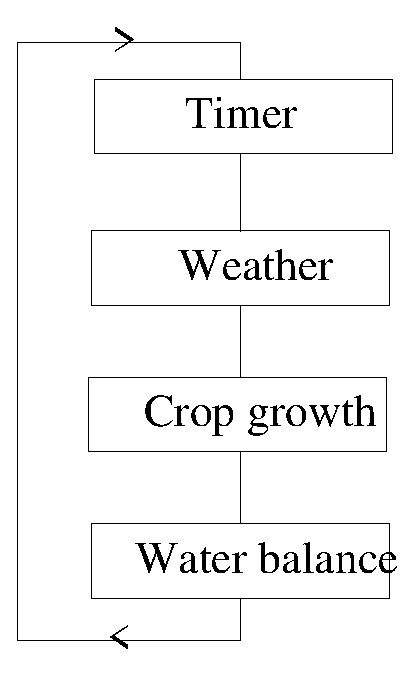
\epsfig{file=\FigDir/DAGLOOP.eps,width=8.04cm} \end{center}
\end{figure}

\bigskip
\bigskip
\bigskip
\bigskip
\bigskip
\bigskip
\bigskip
\bigskip
\bigskip
\bigskip
\bigskip
\bigskip
\bigskip
\bigskip
\bigskip
\bigskip
\nwln
\begin{tabbing}
\hspace{1.27cm}\=\hspace{1.27cm}\=\hspace{1.27cm}\=\hspace{1.27cm}\=%
\hspace{1.27cm}\=\hspace{1.27cm}\=\hspace{1.27cm}\=\hspace{1.27cm}\=%
\hspace{1.27cm}\=\hspace{1.27cm}\=\kill
Fig. 2.1\> \> Daily calculations of the simulation of crop growth
\end{tabbing}

{\bf {\it Timer\/}}\\
In the WOFOST model, the Euler integration method is used to integrate the plant growth
processes over the growing period (i.e. all the time step executed). Therefore, the model
has to update the time and the time related variables each time the daily calcula\-tions are
performed. The subroutine TIMER takes care of this process, it controls the Euler
integration. The Euler integration method itself, is explained in chapter three.

{\bf {\it Weather\/}}\\
The meteorological parameters which are used by the WOFOST model are: maxi\-mum
temperature, minimum temperature, global radiation, windspeed, vapor pressure,
evapotranspiration and rainfall. In the WOFOST model, the Penman method is used to
calculate the evapotr\-anspiration. The weather related calculations of the model are
explained in chapter four.

\bigskip
Concerning the parameters global radiation and rainfall, it should be mentioned that in the
future JRC versions of WOFOST extra options to calculate this variable will be intro\-duced. Presently, in both versions the global radiation will be estimated using the \AA ngs\-tr\"{o}m formula when no actual data are available. The \AA ngs\-tr\"{o}m formula uses the sunshine
duration as input. If this parame\-ter is not available, in the subsequent JRC versions, the
global radiation will be estimated using either the equation proposed by Supit (1994) or
the Hargre\-aves formula (1985). The method developed by Supit, uses cloud cover and
maximum and minimum as input and its accuracy of the estimates comes close to the
accuracy of the \AA ngs\-tr\"{o}m estimates. The Hargreaves formula uses maximum and
minimum temperature only, and the accuracy of the estimates is less then either the \AA ngs\-tr\"{o}m formula or the method proposed by Supit.\\
Presently, the empirical coefficients of the \AA ngs\-tr\"{o}m formula have to be provided by the
user in the general version. In the JRC version these coefficient can be calculated as a
function of the latitude of the meteorological station.

\bigskip
Actual rainfall data are used as input in both versions. In the general version however, it
is also possible to use generated rainfall. For more informa\-tion about the differences
between these versions, one should consult Appendix 5.

\bigskip
\bigskip
{\bf {\it Crop growth\/}}\\
Crop growth depends on the daily net assimilation, which on its turn depends on the
intercepted light. The intercepted light is determined by the level of incoming radiation
and the leaf area of the crop. From the absorbed radiation and the photosynthetic
characteristics of single leaves, the daily rate of potential gross photosynthesis can be
calculated. Reduction of the transpiration due to water or oxygen stress results in a
reduced production of assimilates. The assimilates are partitioned over the various plant
organs. Figure 2.2 presents a diagram of the crop growth processes. Chapter five explains
in detail these processes.

\bigskip
\begin{figure}[htbp]
 \begin{center}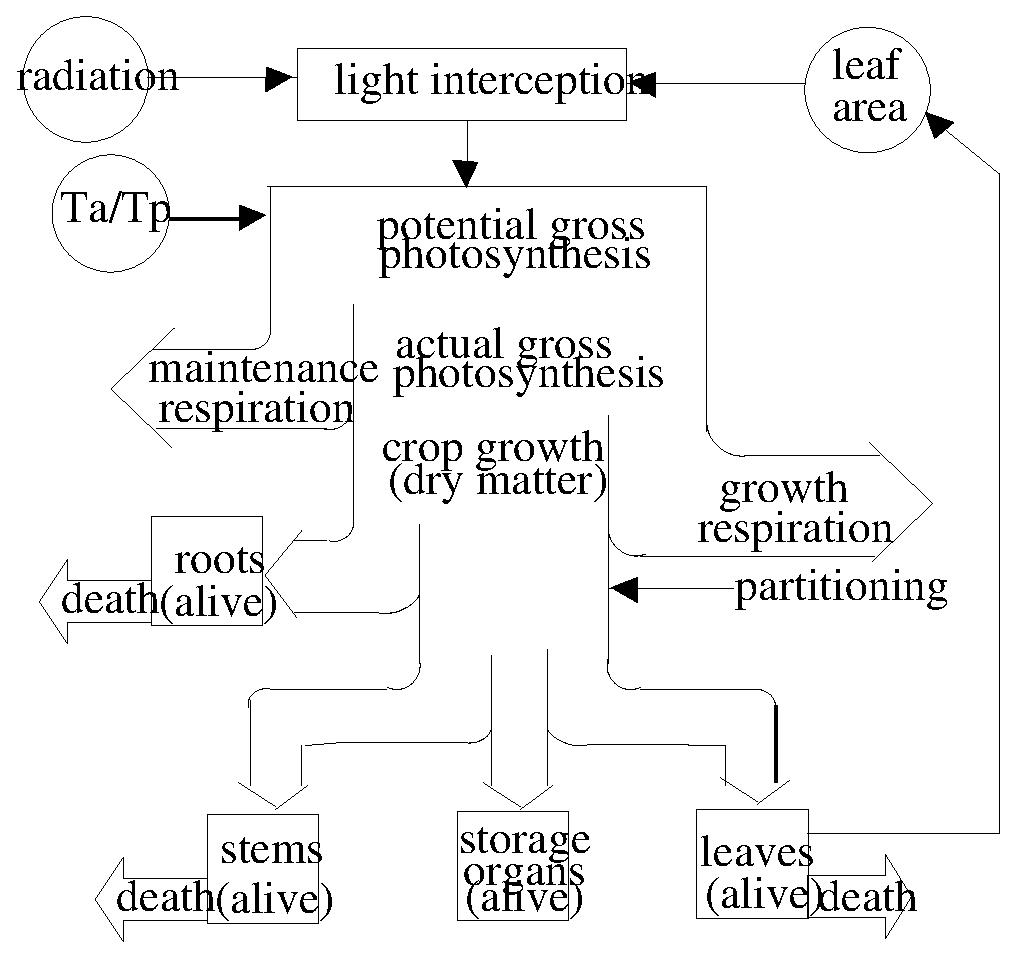
\epsfig{file=\FigDir/ASIMTREE.eps,width=\textwidth} \end{center}
\end{figure}
Fig. 2.2
\testlastline

\begin{indenting}{2.54cm}
Crop growth pro\-cesses. {\small T$_{{\rm a}}$ and T$_{{\rm p}}$ are actual and potential transpiration rate.} (de
Koning, 1993)
\end{indenting}

\bigskip
{\bf {\it Water balance\/}}\\
A crop growth simulation model also has to keep track of the soil moisture content to
deter\-mine when and to what degree a crop is exposed to water stress. This can be done
with the aid of a water balance, which com\-pares for a given period of time, incoming
water in the rooted surface soil with outgoing water and quantifies the difference between
the two as a change in the amount of soil moisture {\nobreak}stored. The WOFOST model distin\-guishes three different situations. The first situation occurs when the soil moisture is at
field capacity and the crop growth reaches its potential level. In the second situation, the
influence of evapo(transpi)rati\-on and percolation on the availability of soil moisture are
considered. Production is dimin\-ished by the reduced availability of soil moisture. In the
last situation not only evapo(transpi)ration and percola\-tion are regarded but also influence
of groundwater is taken into account. Figure 2.3 illustrates the three possible situations in
the WOFOST model. Detailed information on this subject can be found in chapter six.

\bigskip
\begin{figure}[htbp]
 \begin{center}\epsfig{file=\FigDir/SOILLOOP.eps,width=\textwidth} \end{center}
\end{figure}

\bigskip
\bigskip
\bigskip
\bigskip
\bigskip
\bigskip
  \bigskip
Fig. 2.3
\testlastline

\begin{indenting}{2.54cm}
The three possible situations of the water balance which are distin\-guished
by WOFOST 6.0
\end{indenting}

\bigskip
As mentioned before, the calculations of crop growth simulation are made on a daily
basis, (loop over days). WOFOST does also simulate crop growth for a number of growth
seasons. Only one growth season can be simulated for one cal\-endar year. Figure 2.4
depicts the flow scheme of the yearly calculations (loop over years). The influ\-ence of
nutrients (nitrogen, phos\-phate and potassi\-um) on the yield and the yield statistics are
calculated on a yearly basis.

\bigskip
The procedure which calculates the nutrient requirements is based on the work of Janssen
et al (1990). The routine consist of four successive steps. First the potential supplies of
nitrogen, phosphorus and potassium are calculated, applying relationships between
chemical properties of the soil layer 0-20 cm and the maximum quantity of those nutrients
that can be absorbed by maize. It is assumed that the yield is not limited by nutrients and
growth factors. In the second step, the actual uptake of each nutrient is calculated as a
function of the potential supply of that nutrient, taking into account the potential supply of
the other two nutrients. The third step compromises the establishment of three yield
ranges as depending on the actual uptakes of nitrogen, phosphorus and potassium,
respectively. In step four these yield ranges are combined in pairs, and the yields
estimated for pairs of nutrients are averaged to obtain an ultimate yield estimate.

\bigskip
In the general WOF\-OST version, statis\-tics and the nutrient limited production are
included. In the JRC version of WOFOST 6.0 however, these features are omitted. See
Appendix 5.

\begin{figure}[htbp]
 \begin{center}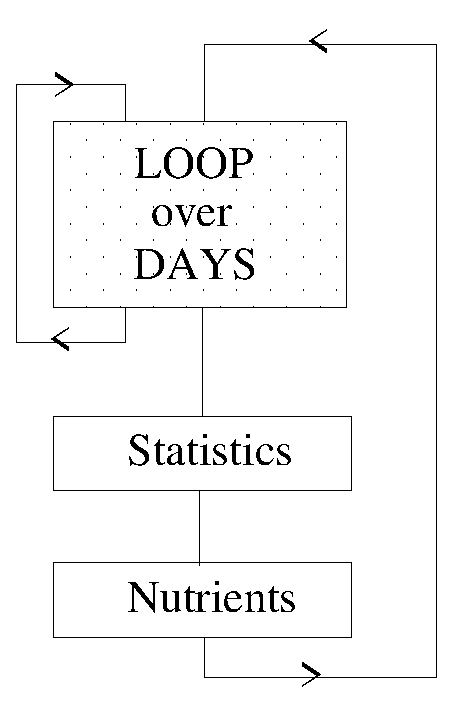
\epsfig{file=\FigDir/JAARLOOP.eps,width=8.04cm} \end{center}
\end{figure}

\bigskip
\bigskip
\bigskip
\bigskip
\bigskip
\bigskip
\bigskip
\bigskip
\bigskip
\bigskip
\bigskip
\bigskip
\bigskip
\bigskip
\bigskip
\bigskip
\bigskip
\nwln
\begin{tabbing}
\hspace{1.27cm}\=\hspace{1.27cm}\=\hspace{1.27cm}\=\hspace{1.27cm}\=%
\hspace{1.27cm}\=\hspace{1.27cm}\=\hspace{1.27cm}\=\hspace{1.27cm}\=%
\hspace{1.27cm}\=\hspace{1.27cm}\=\kill
Fig. 2.4\> \> Yearly calculations of the WOFOST model
\end{tabbing}


\chapter{three}

% This file was created by the WP2LaTeX program version: 3.51 
\documentclass[11pt]{report}
\usepackage{wp2latex}
\usepackage{InputPS}
\usepackage[USenglish]{babel}
\usepackage{amsmath}
\usepackage{tabularx}

\newcommand{\FigDir}{.}
\ShowDisplacementBoxes

\begin{document}
\chapter{one}
\chapter{two}
\chapter{three}
\chapter{WEATHER}

Subroutine {\bf PENMAN} calculates the potential evapotranspiration of a crop canopy, bare
soil and a water surface. Some intermediate variables, used in the calculation are also
computed.

\section{Calculation of evapotranspiration}

Strictly speaking, transpiration is the loss of water from the plants, and evaporation is the
loss of water from the soil or from a free-water surface. Evapotranspiration covers both
transpiration and evaporation.
The principal driving force for evaporation is the gradient of vapor pressure between the
evaporating surface and the surrounding air. The vapor pressure at the evaporating
surface is equal to the saturated vapor pressure at the prevailing temperature of that
surface. The vapor pressure of the air is a function of the ambient temperature and its
relative humidity. The rate of evaporation depends on the diffusion resistance between the
evaporating surface and the air.
The magnitude of the resistance is strongly related to wind speed. The two environ\-mental
variables, air humidity and wind speed combined determine the 'evaporative demand' of
the air.

The problem in the approach above is that the temperature of the evaporating surface is
usually not known from standard meteorological observations. Evaporation  of 1 mm
layer of water requires 2.4 MJ m$^{{\rm -2}}$ of energy and can therefore be described through
quantification of an energy balance. The energy dissipation, required for evaporation,
leads to cooling of the evaporating surface which reduces the vapor gradient. Hence, a
driving force is required to maintain the corresponding surface temperature, and thus,
maintain the vapor pres\-sure gradient. The energy for this driving force is supplied by the
net solar radiation received by the canopy and or soil.\\
Net radiation is the balance between incoming (short-wave) radiation from the sun and
radiation losses due to reflection and outgoing (long-wave) radiation. Heat supplied by
moving air is another source of energy, but this is usually negligible, except in situations
where the vegetation is surrounded by extensive bare areas (oasis). Only 5-8\% of
incoming radiation is dissipated in photosynthesis, which is, therefore, disregarded here.
Respiration yields an insignificant amount of energy. To simplify the treatment of
evapotranspiration, it is considered to be governed by two factors: radiation and evaporative demand.

Penman (1948) was the first to describe evapotranspiration in physi\-cal mathematical
terms. He calculated evaporation from free-water surfaces, wet bare soil and low grass
swards for 10-day periods. There is ongoing discussion in the literature whether his
formulae are also applicable if daily values are used. If used with daily values, 24 hour
average values should be used. For large day/night differences (e.g. in wind speed),
Dooren\-bos \& Kassam (1979) suggested the use of correction factors.\\
The value calculated according to the Penman equations is the potential evapo\-{\nobreak}transpiration, i.e. without limitations with respect to the supply of liquid water to the
evaporating surface. This ET0 (Penman) value is often used as a reference value, to
which actual crop water demand is related. To translate ET0 into crop water require\-ments,
 so called crop factors can be used (e.g. Doorenbos \& Pruitt, 1977; Feddes {\it et al.\/},
1978). See also \S 6.1.

The Penman formula (equation 4.1) consists of two segments. The first part, the radiative
term, calculates the net absorbed radiation. The second part, the aerodynamic term,
calculates the evapora\-tive demand of the atmo\-sphere (Choisnel {\it et al\/}., 1992; Fr\`{e}re and
Popov, 1979; Penman, 1956, 1948). The resulting equations are used to calculate the
potential evapora\-tion rates from a water surface, from bare soil surfaces and the potential
evapotranspira\-tion rate from a crop canopy.


\begin{equation}
\label{eqET0}
ET0 ~=~ W ~R _{na} ~+~(1\, -\, W) ~E _{a} 
\end{equation}

Where:\\
\begin{tabularx}{\textwidth}{llXr}
ET0&:& Evapo(transpi)ration & [mm d$^{{\rm -1}}$] \\
W&:& Temperature related weighing factor &  [-] \\
R$_{{\rm na}}$&: & Net absorbed radiation in equivalent evaporation & [mm d$^{{\rm -1}}$] \\
EA&: &  Evaporative demand in equivalent evaporation & [mm d$^{{\rm -1}}$] \\
\end{tabularx}

\subsection{Preparatory calculations}

The average temperature is calculated as the average of the minimum and the maximum
tempera\-ture. This average temperature \={T} is equal to the so called air temperature (T) used
in the model calcula\-tions. The maxi\-mum and minimum temperature are measured daily
values.

\begin{equation}
T ~=~{\frac{T _{\max } ~+~ T _{\min } }{2}}
\end{equation}

Where:\\
\begin{tabularx}{\textwidth}{llXr}
T&: & Average daily air temperature & [\degrees C]\\
T$_{{\rm max}}$&:  & Maximum temperature & [\degrees C]\\
T$_{{\rm min}}$&: &  Minimum temperature & [\degrees C]\\
\end{tabularx}


The difference between maximum and minimum temperature is used to calculate the
empiric constant of the wind function in the Penman equation.

\begin{equation}
\Delta T ~= ~T _{\max } ~-~ T _{\min } 
\end{equation}

Where:\\
\begin{tabularx}{\textwidth}{llXr}
$\Delta$T& :& Temperature difference  &[\degrees C]\\
T$_{{\rm max}}$ &:& Maximum temperature &  [\degrees C]\\
T$_{{\rm min}}$& :& Minimum temperature  &[\degrees C]
\end{tabularx}


As will be explained later in \S 4.1.3, the evaporative demand, EA, depends on the 
winds\-peed and the difference between saturated and actual vapor pressure. The windspeed
dependency is incorporated in the evaporative demand as the windspeed  measured at a
height of two meters, and multiplied by an empirical coefficient (see also eq. 4.17). This
coeffi\-cient is tem\-per\-ature dependent and can be calculated as (Fr\`{e}re, 1979):

\begin{eqnarray}
\label{eqBU}
BU ~=~ 0.54 ~+ ~0.35\,{\frac{\Delta T\, -\, 12}{4}} ~~~for~\Delta ~ T~\ge ~ 12 \degrees C \\
\nonumber
BU~=~0.54 ~~~for~\Delta ~ T~<~12 \degrees C
\end{eqnarray}

Where:\\
\begin{tabularx}{\textwidth}{llXr}
BU & :& Empirical coefficient in the wind function &  [-]\\
$\Delta$T& :& Temperature difference & [\degrees C] \\
\end{tabularx}
\hspace*{6em}

The air temperature can be used to calculate the latent heat of vaporization: 

\begin{equation}
{\it \lambda} ~=~ 2.501~ -~ (2.361 \cdot 10^{-3} )\, T
\end{equation}

Where:\\
\begin{tabularx}{\textwidth}{llXr}
$\lambda$& :& Latent heat of vaporization & [MJ kg$^{{\rm -1}}$]\\
T &:& Average daily temperature & [\degrees C]\\
\end{tabularx}


As the value of the latent heat varies only slightly over normal temperature ranges a
single value for $\lambda$ may be taken. In the model for $\lambda$ a value of 2.45 MJ kg$^{{\rm -1}}$ is assumed (T=20\degrees C). The barometric pressure at sea level is used to calculate the psychrometric constant at sea level (Brunt, 1932).

\begin{equation}
\gamma _{o} ~=~ {{\frac{\it C _{p} \, P _{o} }{{\it  \epsilon \, \lambda } }} }\, 10 ^{-3} ~=~ 0.00163\,{\it P} _{\frac{o}{\it \lambda}} 
\end{equation}

Where:\\
\begin{tabularx}{\textwidth}{llXr}
$\gamma$$_{{\rm o}}$ & :& Psychrometric constant at sea level & [kPa \degrees C$^{{\rm -1}}$]\\
C$_{{\rm p}}$ & :& Specific heat of moist air = 1.013 10$^{{\rm -3}}$ & [MJ kg$^{{\rm -1}}$ \degrees C$^{{\rm -1}}$]\\
P$_{{\rm o}}$ & :& Atmospheric pressure at sea level & [kPa]\\
$\epsilon$ & :& Ratio molecule weight water vapor / dry air = 0.622 & []\\
$\lambda$ & :& Latent Heat of vaporization & [MJ kg$^{{\rm -1}}$]\\
\end{tabularx}


 In the model however, a fixed value of $\gamma$$_{{\rm o}}$ = 0.67 is assumed. This value can be obtained by using for P the atmospheric pressure at sea level, which is assumed to be 101.3 kPa and $\lambda$ = 2.45 MJ kg$^{{\rm -1}}$. It should be mentioned, that the barometric pressure changes with altitude, so does also the psychrometer constant. Therefore, the two following equations are used to correct for altitude difference.

\begin{equation}
P~=~P _{o} \, e ^{{\frac{-0.034\, z}{T\, +\, 273}} }
\end{equation}

Where:\\
\begin{tabularx}{\textwidth}{llXr}
P &:& Atmospheric pressure at elevation z  & [kPa]\\
P$_{{\rm o}}$ &:& Atmospheric pressure at sea level  & [kPa]\\
T &:& Daily temperature  & [\degrees C]\\
z &:& Elevation  & [m]
\end{tabularx}

\begin{equation}
\label{eqPsycho}
\gamma ~=~ \gamma _{o} \,{\frac{P}{P _{o} }}
\end{equation}

Where:\\
\begin{tabularx}{\textwidth}{llXr}
$\gamma$ &:& Psychrometric constant at elevation z & [kPa \degrees C]\\
$\gamma$$_{{\rm o}}$ &:& Psychrometric constant at sea level & [kPa \degrees C]\\
P &:& Atmospheric pressure at elevation z & [kPa]\\
P$_{{\rm o}}$ &:& Atmospheric pressure at sea level & [kPa]\\
\end{tabularx}

The saturated vapor pressure is related to the mean daily air temperature and may be
approxi\-mated with the equation of Goudriaan (1977). 

\begin{equation}
\label{eqSVP}
e_{s} ~=~ 0.610588\, \cdot \, e ^{{\frac{17.32491\, T}{T\, +\, 238.102}} }
\end{equation}

Where:\\
\begin{tabularx}{\textwidth}{llXr}
e$_{{\rm s}}$ &:& Saturated vapor pressure  & [kPa]\\
T &:& Air temperature & [\degrees C]
\end{tabularx}

From this equation the derivate, i.e. the slope of the saturated vapor pressure-temperature
curve is established.

\begin{equation}
\label{eqSlopeSVP}
\Delta ~=~{\frac{238.102 \cdot 17.32491 \cdot e_{s} }{(T + 238.102)^{2} }}
\end{equation}

Where:\\
\begin{tabularx}{\textwidth}{llXr}
$\Delta$ &:& Slope of the saturation vapor pressure curve  & [kPa \degrees C$^{{\rm -1}}$]\\
e$_{{\rm s}}$ &:& Saturated vapor pressure &  [kPa]\\
T &:& Air temperature & [\degrees C]
\end{tabularx}

The measured vapor pressure is not allowed to exceed the calculated saturated vapor
pressure.
 
\subsection{Methods to estimate global radiation}

In case no observations for the incoming solar radiation are available, the formula
postulated by \AA ngstr\"{o}m (1924) can be used to estimate this parameter using sunshine
duration observations.

\begin{equation}
\label{eqGlobRad}
S _{g,d} ~=~S _{o,d} \, (A\, +\, B\,{\frac{n}{D}} )
\end{equation}

Where:\\
\begin{tabularx}{\textwidth}{llXr}
S$_{{\rm g,d}}$ &:& Incoming daily global solar radiation  & [J m$^{{\rm -2}}$ d$^{{\rm -1}}$]\\
S$_{{\rm o,d}}$ &:& Daily extra-terrestrial radiation (see eq. 4.27)  & [J m$^{{\rm -2}}$ d$^{{\rm -1}}$]\\
A &:& Empirical constant  & [-]\\
B &:& Empirical constant  & [-]\\
n &:& Bright sunshine hours per day  & [hr]\\
D &:& Astronomical day length (see e.q. 4.25)  & [hr]
\end{tabularx}

t should be mentioned that the empirical constants A and B of the \AA ngstr\"{o}m formula can be found with linear regression by comparing the incoming global radiation with the
relative sunshine duration n/D, taking into consideration the daily extra-terrestrial
radiation. A is the intercept and B the slope of the regression. It should also be mentioned
that the regression constants A and B have a physical meaning. A can be considered as
the fraction of extra terrestrial radiation on overcast days. The sum of A and B can be
considered as the fraction of radiation received on clear days.\\
For several regions in Europe the \AA ngstr\"{o}m constants have been established by Supit
(1994). Indicative values for empirical constants in the \AA ngstr\"{o}m formula are depicted in Table \ref{tab:angstAB}.

\begin{table}
\caption{Indicative values for empirical constants in the \AA ngstr\"{o}m formula in
relation to latitude and climate used by the FAO (Fr\`{e}re \& Popov, 1979)}
\label{tab:angstAB}
\begin{tabular}{lcc}
\hline
Zone &   A &  B                \\
\hline
Cold and temperate zones   &  0.18 &  0.55\\
Dry tropical zones  &   0.25  & 0.45\\
Humid tropical zones  &   0.29 &  0.42\\
\hline
\end{tabular}
\end{table}

It should be clear that the constants {\bf A} and {\bf B} (acronym: {\bf COEFA} and {\bf COEFB}) should be
provided by the user. However, in case these constants are not available, in the JRC
version of WOFOST 6.0 (in subrou\-tine {\bf METEO}), the following approximation is used:

\begin{eqnarray*}
 A~=~0.4885~-~0.0052 \, LAT \\
 B~=~0.1563~+~0.0074 \, LAT 
\end{eqnarray*}

Where:\\
\begin{tabularx}{\textwidth}{llXr}
A &:& Empirical constant  & [-]\\
B &:& Empirical constant  & [-]\\
LAT &:& Latitude  & [degrees]\\
\end{tabularx}

As an improvement, in future versions of WOFOST, the method developed by Supit
(1994) will be introduced in the model. This method calculates the incoming global
radiation as a function of cloud cover and sunshine duration. It can be considered as an
extension of the formula developed by Hargreaves (1985). 
Using this method, the accuracy of the results is slightly less in comparison to the results obtained with the \AA ngstr\"{o}m formula.

\begin{equation}
S _{g,d} ~=~ c _{a} \, S _{o,d} \, (\sqrt{(T _{\max} ~-~T _{\min} )} ~+~ c _{b} \sqrt{(1-{Cloud/8})} ~) ~+~c _{c} 
\end{equation}

Where:\\
\begin{tabularx}{\textwidth}{llXr}
S$_{{\rm g,d}}$ &:& Incoming daily global solar radiation  & [J m$^{{\rm -2}}$ d$^{{\rm -1}}$]\\
S$_{{\rm o,d}}$ &:& Daily extra-terrestrial radiation (see eq. 4.27)  & [J m$^{{\rm -2}}$ d$^{{\rm -1}}$]\\
Cloud &:& Mean total cloud cover during daytime  & [octas]\\
T$_{{\rm max}}$ &:& Maximum temperature  & [\degrees C]\\
T$_{{\rm min}}$ &:& Minimum temperature  & [\degrees C]\\
c$_{{\rm a}}$,c$_{{\rm b}}$,c$_{{\rm c}}$ &:& Empirical regression constants   & [-]
\end{tabularx}

For five regions in Europe the constants c$_{{\rm a}}$, c$_{{\rm b}}$ and c$_{{\rm c}}$ have been established (Supit, 1994).

As a second improvement, the Hargreaves formula (1985) will be introduced in the
model. In case no observa\-tions of either incoming radiation, sunshine duration and
cloudco\-ver are available, this formula, will be used. The accuracy of this method is less
then the accuracy of the two earlier mentioned methods.

\begin{equation}
S _{g,d} ~=~ c _{d} \, S _{o,d} \, \sqrt{(T _{\max} ~-~T _{\min} )} ~+~c _{e} 
\end{equation}

Where:\\
\begin{tabularx}{\textwidth}{llXr}
S$_{{\rm g,d}}$ &:& Incoming daily global solar radiation  & [J m$^{{\rm -2}}$ d$^{{\rm -1}}$]\\
S$_{{\rm o,d}}$ &:& Daily extra-terrestrial radiation (see eq. 4.27)  & [J m$^{{\rm -2}}$ d$^{{\rm -1}}$]\\
T$_{{\rm max}}$ &:& Maximum temperature  & [\degrees C]\\
T$_{{\rm min}}$ &:& Minimum temperature  & [\degrees C]\\
c$_{{\rm d}}$,c$_{{\rm e}}$  &:& Empirical regression constants  & [-]\\
\end{tabularx}

For six regions in Europe the constants c$_{{\rm d}}$ and c$_{{\rm e}}$ have been established (Supit, 1994). In section \ref{sec:daylength} it is explained how the daily extra-terrestrial radiation, S$_{{\rm o,d}}$, can be calculat\-ed.

\subsection{Terms in the Penman formula  }

The temperature related weighing factor W in equation \ref{eqET0} is defined as (Fr\`{e}re andPopov, 1979; Penman, 1948, 1956).

\begin{equation}
W ~=~{\frac{\Delta}{(\Delta ~+~ \gamma )}} 
\end{equation}

Where:\\
\begin{tabularx}{\textwidth}{llXr}
$\Delta$ &:& Slope of the saturation vapor pressure curve (see eq. \ref{eqSlopeSVP})  & [kPa \degrees C$^{{\rm -1}}$]\\
$\gamma$ &:& Psychrometric constant (see eq. \ref{eqPsycho})  & [kPa \degrees C$^{{\rm -1}}$]
\end{tabularx}

To calculate net outgoing long wave radiation Penman (1956) used an equation which is
derived from the formula postulated by Brunt (1932). The net outgoing long wave
radiation increases with increasing values for the mean air temperature and the relative
sunshine duration and decreases with increasing vapor pressure.

\begin{equation}
R _{nl} \uparrow  ~=~ \sigma \,\, (T+273) ^{4} \,\, (0.56\,\, -\,\, 0.079\, \sqrt{e _{a} } )\,\, (0.1\,\, +\,\, 0.9\,\,{\frac{n}{D}} )
\end{equation}


Where:\\
\begin{tabularx}{\textwidth}{llXr}
R$_{{\rm nl}}$$\uparrow$ &:& Net outgoing long-wave radiation & [J m$^{{\rm -2}}$ d$^{{\rm -1}}$]\\
$\sigma$ &:& Stefan Boltzm\-ann constant = 4.90 x 10$^{{\rm -9}}$ & [J m$^{{\rm -2}}$ K$^{{\rm -4}}$ s$^{{\rm -1}}$]\\
T &:& Air temperature & [\degrees C]\\
e$_{{\rm a}}$ &:& Actual vapor pressure & [kPa]\\
n/D &:& Relative sunshine duration & [-]\\
\end{tabularx}

The relative sunshine duration, n/D, is established in the model using:

\begin{equation}
{\frac{n}{D}} ~=~{\frac{T _{atm} ~-~A}{B}}
\end{equation}

Where:\\
\begin{tabularx}{\textwidth}{llXr}
n/D &:& Relative sunshine duration  & [-]\\
T$_{{\rm atm}}$ &:& Atmospheric transmission (see eq. 4.29)  & [-]\\
A &:& Empirical constant in the \AA ngstr\"{o}m equation  & [-]\\
B &:& Empirical constant in the \AA ngstr\"{o}m equation  & [-]\\
\end{tabularx}


The calculation of the atmospheric transmission, T$_{{\rm atm}}$, will be explained in 4.2.

Part of the actual received radiation is reflected by the surface. The fraction reflected
(albedo) is different for a water surface, a soil surface and a crop canopy. The absorbed
fraction of radiation actually received minus the net outgoing radiation equals the net
absorbed radiation, which is divided by the latent heat of vaporization of water to express
the amount of radiation in depth of evaporative water layer (mm d$^{{\rm -1}}$).

\begin{equation}
\label{eqAbsGlobRad}
R _{na} ~=~{\frac{(1\, -\, \alpha )\,\, R _{av} \, -\, R _{nl} \uparrow  }{\lambda}}
\end{equation}

 
Where:\\
\begin{tabularx}{\textwidth}{llXr}
R$_{{\rm na}}$ &:& Net absorbed radiation  & [mm d$^{{\rm -1}}$]\\
$\alpha$ &:& Albedo or reflection coefficient of regarded surface  & [-]\\
R$_{{\rm av}}$ &:& Average radiation  & [J m$^{{\rm -2}}$ d$^{{\rm -1}}$]\\
R$_{{\rm nl}}$$\uparrow$ &:& Net outgoing long-wave radiation  & [J m$^{{\rm -2}}$ d$^{{\rm -1}}$]\\
$\lambda$ &:& Latent heat  & [J kg$^{{\rm -1}}$]\\
\end{tabularx}


The soil's albedo depends on the surface color and on the moisture content. Albedo
values for dry soil vary from 0.14 (clay) to 0.37 (dune sand). Ten Berge (1986) described
the depen\-dence of the albedo value on soil moisture in relation to the average water
content of the top soil layer. See Table \ref{tab:AlbedoSoils}. \\
In WOFOST Version 6.0 the following values for the albedo are assumed: for bare soil
0.15, for a canopy  0.25 and for a water surface a value of 0.05.

\begin{table}
\caption{Albedo values for wet and dry soils (ten Berge, 1986)}
\label{tab:AlbedoSoils}
\begin{tabular}{lcc}
\hline
soil type & wet & dry\\
\hline
Dune sand  &   0.24 &  0.37 \\
Sandy loam &    0.10-0.19 &  0.17-0.23\\
Clay loam &    0.10-0.14 &  0.20-0.23\\
Clay &    0.08 &  0.14\\
\hline
\end{tabular}
\end{table}

The evaporative demand of the atmosphere depends on the difference between saturated
and actual vapor pressure and on the wind function. For crop canopies the evaporative
demand is somewhat higher than for soil or water surfaces due to a higher surface
roughness. This is reflected in a higher value for {\it factor\/} in the wind function.

\begin{equation}
\label{eqEvapDemand}
EA~=~0.26\, (e _{s} \, -\, e _{a} )\,\, (factor\, +\, BU\, u(2))
\end{equation}
 
Where:\\
\begin{tabularx}{\textwidth}{llXr}
EA &:& Evaporative demand  & [mm d$^{{\rm -1}}$]\\
e$_{{\rm s}}$ &:& Saturated vapor pressure (see eq. \ref{eqSVP})  & [kPa]\\
e$_{{\rm a}}$ &:& Actual vapor pressure  & [kPa]\\
{\it factor\/} &:& Empirical constant  & [-]\\
BU &:& Coefficient in wind function (see eq. \ref{eqBU})  & [-]\\
u(2) &:& Mean windspeed at 2 m height  & [m s$^{{\rm -1}}$]
\end{tabularx}

The following values for {\it factor\/} are assumed (Fr\`{e}re, 1979). For crop canopies {\it factor\/} =
1.0 and for a free water a surface {\it factor\/} = 0.5.

Substituting equations \ref{eqEvapDemand} and \ref{eqAbsGlobRad} in equation 4.1 yields

\begin{equation}
\label{eqPenman}
ET0 ~=~{\frac{(\Delta R _{na~} +~\gamma EA)}{\Delta ~+~\gamma }}
\end{equation}

Where:\\
\begin{tabularx}{\textwidth}{llXr}
ET0 &:& Evapo(transpiration)  & [mm d$^{{\rm -1}}$]\\
R$_{{\rm na}}$ &:& Net absorbed radiation  & [mm d$^{{\rm -1}}$]\\
EA &:& Evaporative demand  & [mm d$^{{\rm -1}}$]\\
$\Delta$ &:& Slope of the saturation vapor pressure curve   & [kPa \degrees C$^{{\rm -1}}$]\\
$\gamma$ &:& Psychrometric constant  & [kPa \degrees C$^{{\rm -1}}$]
\end{tabularx}

With the equations \ref{eqAbsGlobRad}, \ref{eqEvapDemand}, \ref{eqPenman} and the different values for factor and albedo, the evapo(transpi)ration from a wet bare soil surface E0$_{{\rm s}}$, a water surface, E0$_{{\rm w}}$, and a crop canopy, ET0, can be easily calculated.

Measured or estimated daily global irradiation (wavelength 300-3000 nm) is input in the
model (R$_{{\rm av}}$=S$_{{\rm g,d}}$ is assumed). It should be mentioned that the dimension of E0$_{{\rm s}}$, E0$_{{\rm w}}$ and ET0 is mm d$^{{\rm -1}}$ in subroutine {\bf PENMAN}. However, in all the other routines the dimension of these variables is cm d$^{{\rm -1}}$. In the routine {\bf METEO} the dimension of E0$_{{\rm s}}$, E0$_{{\rm w}}$ and ET0 is changed to cm d$^{{\rm -1}}$.


\section{Day length and solar elevation}
\label{sec:daylength}

Subroutine {\bf ASTRO} calculates day length, some intermediate variables for the calculation
of the solar elevation, the integral of the solar elevation over a day and the fraction of
diffuse radiation.

Day length is a function of the angle of the sun above the horizon (solar elevation). Solar
elevation is the angle between the sun rays and the earth's surface. Solar elevation is
determined by latitude, the day and the hour on a certain day. \\
The dependency on the hour of a certain day is simple to explain. The sun rises and the
sun sets every day. Just before sun rise and just after sun set the solar elevation is zero. At the equator on days that the sun is in zenith (the point in the sky directly overhead) at 12 o'clock solar time it holds that:

\begin{equation}
\sin \beta = \cos (15(t _{h} -12))
\end{equation}

Where:\\
\begin{tabularx}{\textwidth}{llXr}
$\beta$ &:& Solar elevation  & [degrees]\\
t$_{{\rm h}}$ &:& Hour of the day  & [h]\\
\end{tabularx}

The angle of the sun changes during the day because the earth rotates once around its axis
every 24 hours at a speed of 15\degrees  per hour (= 360/24).  

To explain the dependency of solar elevation on latitude and day number first the situation
is regarded when the sun is in zenith. This is at 12 o'clock solar time (not to be mixed up
with noon). The solar declination, the place were the sun is in zenith at 12 o'clock solar
time, changes every day. On the 21$^{\rm st}$ of June the sun stands perpen\-dicular above the northern tropic of Cancer (+23.45\degrees N) and on the 22$^{\rm nd}$ of December the sun stands perpendicular above the tropic of Capricorn (-23.45\degrees S). In figure \ref{fig:solardecl} the situation is depicted for 22$^{\rm nd}$ of December when the sun reaches its highest point at the tropic of Capricorn at the southern hemisphere. On the northern hemisphere this results in the shortest day of the year. \\

\begin{figure}[htbp]
\caption{Solar declination}
\label{fig:solardecl}
\begin{forcewidth}{9.33cm}
 \begin{center}\InputPS{\FigDir/AARDE3.eps} \end{center}
\end{forcewidth}
\end{figure}

The solar {\nobreak}declination during the year can be approached by a cosine function. (Note a shift of ten days).

\begin{equation}
\delta ~=~ -23.45 \cos ( 2 \pi {\frac{t _{d} + 10}{365}} )
\end{equation}

Where:\\
\begin{tabularx}{\textwidth}{llXr}
$\delta$ &:& Solar declination   & [de\-grees]\\
t$_{{\rm d}}$ &:& Number of the day since 1 January   & [-]\\
\end{tabularx}

The distance of the sun to the earth is considered to be infinite, therefore declination can be considered equal for all places on earth. The orbit of the earth around the sun is a non concentric ellipse (see figure \ref{fig:orbit}), therefore the solar radiation received at the top of the atmosphere during the year is not constant. At the first of January the earth is closest to the sun, radiation at the top of the atmosphere will then be higher as during other days. \\

\begin{figure}[htbp]
\caption{Orbit of the earth around the sun}
\label{fig:orbit}
\begin{forcewidth}{7.77cm}
 \begin{center}\InputPS{\FigDir/ELIPS.eps} \end{center}
\end{forcewidth}
\end{figure}

The average solar radiation at the top of the atmosphere is estimated at 1370 W m$^{\rm -2}$. A daily solar radiation constant can than be calculated as a cosine times the average solar radiation at the top of the atmosphere multiplied by correction factor to correct for the elliptical orbit of the earth around the sun. This correction factor is estimated to be 0.033.

\begin{equation}
\label{eq:SolarConst}
S _{c,d} = S _{c} (1+0.033 \cos (2 \pi {\frac{t _{d} }{365}} ))
\end{equation}

Where:\\
\begin{tabularx}{\textwidth}{llXr}
S$_{{\rm c,d}}$ &:& Solar constant at the top of the atmosphere for a certain day  & [J m$^{{\rm -2}}$ s$^{{\rm -1}}$]\\
S$_{{\rm c}}$ &:& Average solar radiation at the top of atmosphere (1370 J m$^{{\rm -2}}$ s$^{{\rm -1}}$; I.E.A., 1978) & [J m$^{{\rm -2}}$ s$^{{\rm -1}}$]\\
t$_{{\rm d}}$ &:& Number of day since 1 January  & [-]\\
\end{tabularx}

Note that during the winter in Europe the solar radiation at the top of the atmo\-sphere is at its maximum!\\
The height of the sun at any moment throughout the day and at any place and date can be
calculated with (subroutine {\bf TOTASS}):

\begin{equation}
\sin \beta = \sin \lambda \sin \delta + \cos \lambda \cos \delta \cos (2 \pi {\frac{(t _{h} +12)}{24}} )
\end{equation}

Where:\\
\begin{tabularx}{\textwidth}{llXr}
$\beta$ &:& Solar elevation  & [degrees]\\
$\lambda$ &:& Latitude  & [degrees]\\
$\delta$ &:& Solar declination  & [degrees]\\
t$_{{\rm h}}$ &:& Hour of the day (solar time)  & [h]\\
\end{tabularx}

To compute day length for photoperiod-sensitive species, it must be realized that, even
when the sun is still below the horizon the light level is high enough to trigger the
photoperiodicity mechan\-ism. Photoperiodic day length is 0.5 h longer than the astronomi\-cal day length at the equator and about 0.8 h in temperate zones, depend\-ing on the date of the year. The light level to which photoperiodism is sensitive is quite low and not well
quantified. Vergara \& Chang (1985) determined it to be 1.5-15 mW m$^{{\rm -2}}$ for rice crops; Salisbury (1981) determined the level to be higher. As a compromise a value of 50 mW
m$^{{\rm -2}}$ is used in the model, which corresponds with a sun angle of -4 degrees. The
photosynthetic active period and the astro\-nomical day length can be calculated as:

\begin{equation}
D ~=~ 12~+~{\frac{24}{180}} \, \arcsin \, (\,{\frac{-\sin {\frac{p}{180}} + sinLD}{cosLD}} )
\end{equation}

Where:\\
\begin{tabularx}{\textwidth}{llXr}
D &:& Day length  & [h]\\
sinLD &:& Seasonal offset of sine of solar height = sin$\delta$sin$\lambda$  & [-]\\
cosLD &:& Amplitude of sine of solar height = cos$\delta$cos$\lambda$  & [-]\\
p &:& correction constant  & [degrees]\\
\end{tabularx}

The correction constant for the photosynthetic day length is -4 degrees. For the astro\-nomical day length the correction constant is -0.833 degrees (i.e. solar height for which
the upper edge of the solar disk appears on the horizon). However, in the model for the
calculation of the astronomi\-cal day length, a correction constant of 0 degrees is used. 

The calculation of the photoperi\-odic day length makes no sense when the sun is continu\-ous\-ly at higher inclinations, therefore this calculation method is limited to -66.5+4 and
66.5-4 degrees of latitude.

 The integral of the solar height over the day can be obtained as twice the integral from
sunrise ($\beta$=0\degrees ) to 12 o'clock solar time ($\beta$ = 90\degrees  + $\delta$ - $\lambda$):

\begin{equation}
\label{eq:IntgrlSolarHeigh}
\int \sin \beta dt _{h} ~=~ 3600( D \sin \lambda \sin \delta +{\frac{24}{\pi }} \cos \lambda \cos \delta \sqrt{1-\tan^{2} \lambda \tan^{2} \delta } )
\end{equation}

Where:\\
\begin{tabularx}{\textwidth}{llXr}
$\int$sin$\beta$  &:& Integral solar height & [s]\\
D  &:& Day length & [h]\\
$\beta$  &:& Solar elevation & [degrees]\\
t$_{{\rm h}}$  &:& Hour of the day & [h]\\
\end{tabularx}

Multiplication of equation \ref{eq:SolarConst} with \ref{eq:IntgrlSolarHeigh} yields the daily extra-terrestrial radiation which is also known as the Angot radiation. Note that the dimension of the daily extra-terrestrial is radiation J m$^{{\rm -2}}$ d$^{{\rm -1}}$.

\begin{equation}
\label{eq:Angot}
S_{o,d} = S _{c,d} ~ \int \sin \beta dt _{h} 
\end{equation}

Where:\\
\begin{tabularx}{\textwidth}{llXr}
S$_{{\rm o,d}}$ &:& Daily extra-terrestrial radiation  & [J m$^{{\rm -2}}$ d$^{{\rm -1}}$]\\
S$_{{\rm c,d}}$ &:& Solar constant at the top of the atmosphere 
   for a certain day (see eq. \ref{eq:SolarConst}
)  & [J m$^{{\rm -2}}$ s$^{{\rm -1}}$]\\
t$_{{\rm d}}$ &:& Number of day since 1 January  & [-]\\
\end{tabularx}

In the model the integral of the effective solar height, a modification of equation 4.26 is
also calculated. This modified integral takes the effect of the daily course in atmos\-pheric
transmis\-sion into account. Transmission is lower near the margins of the day because of
haze in the morning and clouds in the afternoon. Besides that, path length of solar
radiation in the atmosphere is longer (Spitters {\it et al\/}., 1986). This modified integral can be calculated as:

\begin{align}
\int \sin \beta_{m} &= \int \sin \beta (1+csin \beta ) dt _{h}  \\
                    &=3600(D ( \sin \lambda \sin \delta + 0.4 
                      (( \sin \lambda \sin \delta )^{2} + 0.5( 
                      \cos \lambda \cos \delta ) ^{2} ))  \nonumber \\
                      &\qquad {} +~{\frac{12}{\pi }} \cos \lambda \cos 
                      \delta (2~+~3 ~\times ~ 0.4 \sin \lambda \sin \delta ) 
                      \sqrt{1~-~\tan^{2} \lambda \tan^{2} \delta } ) \nonumber
\end{align}


Where:\\
\begin{tabularx}{\textwidth}{llXr}
$\int$sin$\beta$$_{{\rm m}}$  &:& Integral of effective solar height       & [s]\\
D  &:& Day length       & [h]\\
c  &:& Coefficient of regression on transmission on solar angle = 0.4       & [-]\\
$\beta$  &:& Solar elevation        & [degrees]\\
$\lambda$  &:& Latitude       & [degrees]\\
$\delta$  &:& Solar declination       & [degrees]\\
t$_{{\rm h}}$  &:& Hour of the day       & [h]\\
\end{tabularx}

A distinction is made between diffuse sky light, with incidence under various angles and
direct sunlight with an angle of incidence equal to the solar declination. It is important to distin\-guish these fluxes because of the large difference in illumination intensity between shaded leaves and sunlit leaves and therefore the difference in the CO$_{{\rm 2}}$ assimila\-tion light response of single leaves, which is non-linear. Shaded leaves receive only diffuse radiation. Sunlit leaves receive both direct and diffuse radiation. The diffuse flux is the result of the scattering of sun rays by clouds, aerosols and gases in the atmo\-sphere. The propor\-tion of diffuse light in the total incident light flux depends on the status of the atmosphere, i.e. cloudi\-ness, concentra\-tion of aerosols. This fraction is calculated from the atmospheric transmis\-sion using an empirical function. This relationship is based on data from different meteorologi\-cal stations from a wide range of latitudes and longitudes (Spitters {\it et al\/}., 1986). 

The atmospheric transmission is the ratio between actual radiation and the quantity that
would have reached the earth's surface in the absence of an atmosphere (i.e. Angot
radiation). This ratio can be calculated as:

\begin{equation}
T _{atm} ~=~ s _{\frac{g,d}{S _{c,d} \int \sin \beta }}
\end{equation}

Where:\\
\begin{tabularx}{\textwidth}{llXr}
T$_{{\rm atm}}$ &:& Atmospheric transmission  & [-]\\
S$_{{\rm g,d}}$ &:& Daily global radiation  & [J m$^{{\rm -2}}$ d$^{{\rm -1}}$]\\
S$_{{\rm c,d}}$ &:& Solar constant at the top of the atmosphere for a certain day (see eq.4.23 and 4.27)  & [J m$^{{\rm -2}}$ s$^{{\rm -1}}$]\\
$\int$sin$\beta$  &:& Integral of solar height   & [s]\\
\end{tabularx}

Relationships between the share of the diffuse flux in the global irradiance (S$_{{\rm df}}$/S$_{{\rm g}}$) and the atmospheric transmission (S$_{{\rm g}}$/S$_{{\rm o}}$) are found in several research reports concerning the use
of solar energy in solar collectors. The relation is characterized by an approximately
linear trend for transmissions ranging between 0.35 and 0.75. At low transmissions,
nearly all of the incoming radiation is diffuse so that the curve bends off.\\
There is some variation among published relations, arising from differences in atmos\-pheric conditions, especially relative sunshine duration, water content of the atmosphere,
and cloud type, but also lack of fit of the presented regression equation from the data and
differences in the method of measuring the diffuse radiation.

The relation used in WOFOST Version 6.0 has been derived by de Jong (1980) and has
been recommended by Spitters {\it et al\/}. (1986).

%\begin{eqnarray*}
%{{\frac{S _{df,d} }{S _{g, d} }} ~=~ 1 ~~~~~~~~~~~~~~~~~~~~for ~~~~~~~~~~~{\frac{S _{g,d} }{S _{o,d} }} ~\le ~0.07}  \nonumber  \\
%{{\frac{S _{df,d} }{S _{g,d} }} ~=~ 1-2.3({\frac{S _{g,d} }{S _{o,d} }} -0.07) ^{2} ~~~~for ~~~~0.07~ < ~{\frac{S _{g,d} }{S _{o,d} }} ~\le ~0.35 } \nonumber  \\
%{{\frac{S _{df,d} }{S _{g,d} }} ~=~ 1.33-1.46{\frac{S _{g,d} }{S _{o,d} }} ~~~~~~~for~~~~0.35~ < ~{\frac{S _{g,d} }{S _{o,d} }} ~\le ~ 0.75}  \nonumber  \\
%{{\frac{S _{df,d} }{S _{g,d} }} ~=~ 0.23~~~~~~~~~~~~~~~~ for ~~~~~~~~ ~ ~ ~{\frac{S _{g,d} }{S _{o,d} }} }~>~0.75
%\end{eqnarray*}

\begin{align}
{\frac{S _{df,d} }{S _{g, d} }} &= 1 & 
      for ~~ {\frac{S _{g,d} }{S _{o,d} }} \le 0.07 \nonumber \\
{\frac{S _{df,d} }{S _{g,d} }} &= 1-2.3({\frac{S _{g,d} }{S _{o,d} }} -0.07) ^{2} & 
      for ~~ 0.07 < {\frac{S _{g,d} }{S _{o,d} }} \le 0.35  \nonumber \\
{\frac{S _{df,d} }{S _{g,d} }} &= 1.33-1.46{\frac{S _{g,d} }{S _{o,d} }} &
      for ~~ 0.35 < {\frac{S _{g,d} }{S _{o,d} }} \le 0.75 \nonumber \\
{\frac{S _{df,d} }{S _{g,d} }} &= 0.23 &
      for ~~ {\frac{S _{g,d} }{S _{o,d} }} > 0.75 \nonumber \\
\end{align}

Where:\\
\begin{tabularx}{\textwidth}{llXr}
S$_{{\rm df,d}}$ &:& Daily diffuse radiation  & [J m$^{{\rm -2}}$ d$^{{\rm -1}}$]\\
S$_{{\rm g,d}}$ &:& Daily global radiation  & [J m$^{{\rm -2}}$ d$^{{\rm -1}}$]\\
S$_{{\rm o,d}}$ &:& Daily extra-terrestrial radiation (see eq. \ref{eq:Angot})  & [J m$^{{\rm -2}}$ d$^{{\rm -1}}$]\\
\end{tabularx}

The relationships are remarkably constant over climates and latitudes so that the presented
equations will be valid for a wide range of conditions (Spitters {\it et al\/}., 1986).

Measured or estimated daily total solar irradiation (wavelength 300-3000 nm) is input for
the model. Only half of this incoming radiation is photosynthetical active (PAR,
{\nobreak}Photosynthetical active radiation, wavelength 400 - 700 nm). The photosynthetical active
diffuse radiation, perpendicular to the direction of the solar rays can be calculated as:

\begin{equation}
D _{p} ~=~ S _{\frac{df,d}{S _{g,d} }} ~~ T _{atm} ~0.5S _{c,d} 
\end{equation}

 
Where:\\
\begin{tabularx}{\textwidth}{llXr}
D$_{{\rm p}}$ &:& Diffuse irradiation perpendicular to the direction of light  & [J m$^{{\rm -2}}$ s$^{{\rm -1}}$]\\
T$_{{\rm atm}}$ &:& Atmospheric transmission (see eq. 4.29)  & [-]\\
S$_{{\rm c,d}}$ &:& Solar constant at the top of the atmosphere for a certain day  & [J m$^{{\rm -2}}$ s$^{{\rm -1}}$]\\
S$_{{\rm g,d}}$ &:& Daily global radiation  & [J m$^{{\rm -2}}$ d$^{{\rm -1}}$]\\
S$_{{\rm df,d}}$ &:& Daily diffuse radiation (see eq. 4.30)  & [J m$^{{\rm -2}}$ d$^{{\rm -1}}$]\\
\end{tabularx}

\end{document}

\chapter{CROP}

\section{Overview of the crop growth model}

The WOFOST model describes phenological development, growth and yield forma\-tion of
a crop from emergence till maturity on the basis of crop genetic properties and environ\-mental conditions. The model simulates dry matter accumulation of a crop as a function
of irradiation, temperature and crop characteristics in time steps of one day. 
The basis for calculating dry matter production, is the rate of gross CO$_{{\rm 2}}$ assimilation of
the canopy. This rate is dependent on the radiation energy absorbed by the canopy, which
is a function of incoming radiation and of crop leaf area. From the absorbed radiation and
the photosynthetic characteristics of single leaves, the daily rate of CO$_{{\rm 2}}$ assimilation of the
crop is calculated. Part of the carbohydrates produced (CH$_{{\rm 2}}$O) are used to provide energy
for the maintenance of the existing live biomass (maintenance respiration). The remaining
carbohydrates are converted into structural matter. In this conversion, some of the weight
is lost as growth respir\-ation. The growth rate is thus obtained as:

\begin{equation}
\Delta W ~=~ C _{e} ~( A ~-~ R _{m} )
\end{equation}

 
Where:\\
\begin{tabularx}{\textwidth}{llXr}
$\Delta$W &:& Growth rate    &   [kg Dry Matter ha$^{{\rm -1}}$ d$^{{\rm -1}}$]\\
A  &:& Gross assimilation   rate &  [kg CH$_{{\rm 2}}$O ha$^{{\rm -1}}$ d$^{{\rm -1}}$]\\
R$_{{\rm m}}$  &:& Maintenance respiration rate    &  [kg CH$_{{\rm 2}}$O ha$^{{\rm -1}}$ d$^{{\rm -1}}$]\\
C$_{{\rm e}}$ &:& Conversion efficiency off assimilates total crop   &   [kg Dry Matter kg$^{{\rm -1}}$ CH$_{{\rm 2}}$O]\\
\end{tabularx}

The dry matter produced is partitioned amongst the various plant organs such as roots,
leaves, stems and storage organs, using partitioning factors that are a function of the
phenological development stage of the crop (Spitters et al., 1989). The fraction partioned
to the leaves, determines leaf area development and hence the dynamics of light intercep\-tion. 
The dry weights of the plant organs are obtained by integrating their growth rates
over time (see eq. 3.1).

Leaf mass is subdivided into age classes. During the development of the crop a part of
living biomass dies due to senescence. Some simulated crop growth processes are
influenced by temperature, like for example the maximum rate of photosyn\-thesis and the
maintenance respiration. Other processes like the partitioning of assimilates or decay of
crop tissue are steered by the pheno\-log\-ical stage. The phenological development stage is
calculated as a function of ambient temperature and possibly modified by the effect of day
length. An overview of all these processes was depicted in figure 2.2 (\S 2.1), which is
repeated here below for easy reference. See figure 5.1.

The simulation of phenological development and biomass formation is performed in
subroutine {\bf CROPSI} (general version) or {\bf CRSIM} (JRC version). The simulated process\-es
include the rate of pheno\-logical develop\-ment, CO$_{{\rm 2}}$ assimilation, mainte\-nance respiration,
dry matter partition\-ing resulting in biomass accumulation, growth and senescence of
leaves, transpiration and extension of roots. 

Elaborate calculations of rates of change are performed in specific subroutines called by
{\bf CROPSI} or {\bf CRSIM}. These routines are {\bf TOTASS} and {\bf ASSIM} for the daily assimilation
rate and {\bf EVTRA} for the evapotranspiration rates. All the equations used to describe these
processes are treated in the following sections.

\begin{figure}[htbp]
\caption{Crop growth pro\-cesses. {\small T$_{{\rm a}}$ and T$_{{\rm p}}$ are actual and potential 
transpiration rate.} (deKoning, 1993)}
 \begin{center}\InputPS{\FigDir/ASIMTREE.eps} \end{center}
\end{figure}

\section{Phenological development of a crop}

The physio\-logical age of a plant is defined by the development stage, which on its turn is
characterized by the forma\-tion of the various organs and their appear\-ance. The most
important phenological change is the one from vegetative to the reproduc\-tive stage, which
determines the most important change in the dry matter allocation over organs. As many
physiologi\-cal and morphological processes change with the phenological stage of the
plant, accurate quantification of phenological development is essential in any simulation
model for crop growth. For many annual crops, the development stage can conveniently
be expressed in a dimensionless variable, having the value 0 at seedling emergence, 1 at
flowering and 2 at maturity (van Heemst {\it et al.}, 1986a; 1986b). 

\subsection{Crop emergence  }

As start of the growing season the date of sowing or of emergence can be chosen. For a
photosynthesis-driven model like WOFOST, the simulation of crop growth starts at
emergence. If the sowing date is chosen by the model user, the day of emergence is
determined by the model in subroutine {\bf CROPSI} or {\bf CRSIM}. The crop emer\-gence can be
defined as a function of the effective daily temperature sum since sowing date. Emergence
takes place when the effective daily temperature sum reaches the threshold temperature
for emergence (acronym: {\bf TSUMEM}). This threshold temperature is crop specific and
should be given by the user. The daily effective temperature depends on the base
tempera\-ture, below which no phenologi\-cal process\-es take place, and the maximum daily
tempera\-ture, beyond which the phenological activity does not increase anymore, are also
crop specific. An example of this effective daily tempera\-ture as a function of daily
average temperature is depicted in figure 5.2.

\begin{figure}[htbp]
% fig 5.2
\caption{Effective temperature from sowing to emergence}
 \begin{center}\InputPS{\FigDir/TEFFMAX.eps} \end{center}
\end{figure}

The following relationship can be defined for the effective temperature sum:

\begin{align}
T_{e} &= 0            & T \le T _{b} \nonumber  \\
T_{e} &= T~-~ T _{b}  & T _{b} ~<~T ~ < ~T _{\max ,e} \nonumber  \\
T_{e} &= T _{\max ,e} & T _{b} T \ge  T _{\max \, ,\, e}
\end{align}

Where:\\
\begin{tabularx}{\textwidth}{llXr}
T$_{{\rm e}}$ &:& Effective daily tempera\-ture & [\degrees C]\\
T$_{{\rm max,e}}$ &:& Maximum temperature beyond which phenological 
   activity does not increase    &    [\degrees C]\\
T$_{{\rm b}}$ &:& Base temperature below which phenological development stops & [\degrees C]\\
T  &:& (Average) daily temperature & [\degrees C]
\end{tabularx}

The base temperature, {\bf T$_{{\rm b}}$} (acronym: {\bf TBASEM}), is defined as the lower threshold
tempera\-ture below which phenological activity stops. It is a crop specific variable and
should be provided by the user. The maximum temperature beyond which phenological
activity does not increase, {\bf T$_{{\rm max,e}}$} (acronym: {\bf TEFFMX}) is also crop specific and should be
given by the user. Species originat\-ing from temperate regions show a base temperature of
0$-$3\degrees C, while species of sub\-tropical and tropical origins have a base temperature of
9$-$14\degrees C (Angus {\it et al.\/}, 1981). Within a species, cultivars may vary substantially in their
temperature requirements. The tempera\-ture sum, therefore, must be characterized for
each cultivar or group of cultivars (maturity classes).   

As mentioned earlier, the start of the growing season can be either the sowing date or the
day of emergence. If the sowing date is chosen, it should be provided by the user or it
can be calculated by the model (see Appendix 4).

\subsection{Phenological development stage}

The phenological development rate and development stage are calculated in subrou\-tine
{\bf CROPSI} or {\bf CRSIM}. A crop passes through successive phenological development stages.
The length of these stages depends on the development rate. Development rates before
and after anthesis are controlled day length and/or tempera\-ture. In the model before
anthesis, both factors, temperature and day length, can be active. After anthesis only
temperature influence is possible.\\
Temperature is the main environmental factor affecting the development rate. Higher
temperatures accelerate the development rate leading to shorter growing periods. This rate
responds to temperature according to a curvilinear relationship. However, it has often
been demonstrated, that over a wide range of temperatures, the develop\-ment rate
increases more or less linearly with temperature (van Dobben, 1962; van Keulen \&
Seligman, 1987).

The development rate (for most crops) is expressed on a numerical scale that ranges from
0 to 2, with 0 being emergence, 1 anthesis and 2 maturity. The development rate is
defined as that part of the scale that is accumulated per day for a given variety. For
example, if the time lapse between emergence and anthesis is 50 days, the average
development rate during the pre-anthesis phase is 1/50 or 0.02 d$^{{\rm -1}}$. The development stage
can also be related to the temperature sum, expressed in degree days, that is the sum of
daily temperatures over the period emergence-anthesis or anthesis-maturity. 

The develop\-ment rate per day is then the ratio of daily temperature and temperature sum
(van Heemst, 1986a; 1986b). This assumes a propor\-tionality between tempera\-ture and
develop\-ment rate. Howev\-er, its validity is limited.

In the model a more flexible relation is used where the effective increase in tempera\-ture
sum, used for the calculation of the development rate, is dependent on the daily tempera\-ture (Summerfield \& Roberts, 1987). This relation is specified in an AFGEN table, 
allowing to account for non-linearity (lower and upper threshold values and optimum
ranges). The average temperature is the independent variable in the AFGEN table (see
Appendix 2). The development rate can thus be obtained by:

\begin{equation}
D _{r\, ,\, t} ~=~{\frac{DT _{s} }{\sum T _{i} }}
\end{equation}

Where:\\
\begin{tabularx}{\textwidth}{llXr}
D$_{{\rm r,t}}$ &:& Development rate at time step t  & [d$^{{\rm -1}}$]\\
DT$_{{\rm s}}$ &:& Temperature dependent correction factor & [\degrees C]\\
$\sum$T$_{{\rm i}}$ &:& Temperature sum required to complete stage i & [\degrees C d]\\
\end{tabularx}

The temperature dependent correction factor, {\bf DT$_{{\rm s}}$} (acronym: {\bf DTSMTB}) and the tempera\-ture sum required to complete stage i, {\bf $\sum$T$_{{\rm i}}$} (acronym: {\bf TSUM1} or {\bf TSUM2}) are crop
dependent and should be provided by the user.

The development stage at time step t is the integral of the development rate over the time
(i.e. time span from emergence to current time step) and can be calculated according to:

\begin{equation}
D _{s,t} ~=~ D _{s\, ,\, t-1} ~+~ D _{r\, ,\, t} \,\Delta t
\end{equation}

Where:\\
\begin{tabularx}{\textwidth}{llXr}
D$_{{\rm s,t}}$ &:& Development stage at time step t    &    [-]\\
D$_{{\rm r,t}}$ &:& Development rate at time step t     &   [d$^{{\rm -1}}$]\\
$\Delta$t &:& Time step   &     [d]\\
\end{tabularx}

For certain species or cultivars, during the vegetative stage (i.e. D$_{{\rm s}}$ $<$ 1), the effect of
day len\-gth should be taken into account. Approaches that describe such effects quantita\-tively are given amongst others by  Weir {\it et al.\/} (1984), Hadley {\it et al\/}. (1984) and Reinink {\it et al.\/} (1986). In the model, a reduction factor for the development rate as a function of the day length is intro\-duced. In case of photosensitivity, this reduction factor should be multiplied with equation 5.3 and can be calculated as:

\begin{equation}
% eq 5.3
f _{red} ~=~{\frac{D ~-~D _{c} }{D _{o} ~-~ D _{c} }} ~~~~~~~~~0~\le ~f _{red} ~\le ~1
\end{equation}

Where:\\
\begin{tabularx}{\textwidth}{llXr}
f$_{{\rm red}}$ &:& Development rate reduction factor as function of day length   &     [-]\\
D &:& Present day length (see eq. 4.25)        [h]\\
D$_{{\rm c}}$ &:& Critical day length for development (lower threshold)    &    [h]\\
D$_{{\rm o}}$ &:& Optimum day length for development (upper threshold)    &    [h]\\
\end{tabularx}

The user should provide information whether the development rate depends on tempera\-ture, on day length or on temperature and day length (acronym: {\bf IDSL}). The critical
daylength, {\bf D$_{{\rm c}}$} (acronym: {\bf DLC}) and the optimum daylength, {\bf D$_{{\rm o}}$} (acronym: {\bf DLO}) are crop depen\-dent and should also be provided by the user. 

Note that in modern cultivars, photosen\-sitivity is much less pronounced than in traditional
cultivars, and that for the purpose of modelling the day length influence can be ignored
by choosing an appropriate temperature sum, which lead to  an equivalent crop life cycle.

The simulation of crop growth stops when the development stage reaches the stage at
which the crop will be harvested (acronym: {\bf DVSEND}). This development stage should be
provided by the user. 

\section{Daily assimilation  } 

Daily dry matter production is the most detailed part of the model. The following steps
can be distinguished and will be described separately:
\begin{itemize}
\item Total daily gross CO2 assimilation rate of the canopy\`[\S 5.3.1]
\item Total instantaneous gross CO$_{{\rm 2}}$ assimilation of the canopy \`[\S 5.3.2]
\end{itemize}
 
The daily rate of CO$_{{\rm 2}}$ assimilation of the crop is driven by the intercepted light and can
be obtained by integrating the total instanta\-neous CO$_{{\rm 2}}$ assimilation rate of the canopy over
the day. The total instantaneous assimilation rate is calculated in subrou\-tine {\bf ASSIM}, the
integra\-tion of the total instantaneous assimilation rate in subrou\-tine {\bf TOTASS}. Both
calcula\-tions make use of the Gaussian integration method (Scheid, 1968), a simple and
fast method of numerical integration. This integration method is explained in Appendix 1.
For calculat\-ing daily total assimilation, this 3-point integration method performs very well
(Goudria\-an, 1986; Spitters, 1986)

\subsection{Total daily gross CO2 assimilation rate of the canopy}

To calculate the total daily gross CO$_{{\rm 2}}$ assimilation rate of the whole canopy, an integra\-tion over time should be performed. Therefore, for given fluxes of photosyntheti\-cally
active radiation, at three different periods of the day, the total instantaneous gross canopy
CO$_{{\rm 2}}$ assimila\-tion rate is computed. Afterwards, the integral of the total instantaneous
gross canopy CO$_{{\rm 2}}$ assimila\-tion rate over time, as a weighted average of the selected three
hours, is calculat\-ed (Gaussian integration, see Appendix 1).

For the calculation of the total instantaneous gross canopy CO$_{{\rm 2}}$ assimilation rate, an
integra\-tion over depth of the gross instantaneous assimilation rate has to be per\-formed.
Therefore, at three different depths in the canopy the gross instanta\-neous assimilation rate
is calculated, whereafter the integral of the gross instantaneous assimila\-tion rate over
depth, as a weighted average of the selected depths, is computed (Gaussian integration,
see Appendix 1)

Integration, to calculate the daily total assimilation, is only necessary if instanta\-neous
assimilation will take place. Instanta\-neous assimila\-tion will be zero if the leaf area index
equals zero (no photosynthetic activity). A second restriction for the integration is the
maximum CO$_{{\rm 2}}$ assimilation rate as a function of development stage, which is crop
dependent. When this maxi\-mum assimila\-tion rate at light saturation equals zero also no
instantaneous assimila\-tion will take place and no integration has to be performed.

As is mentioned before, in order to integrate the gross instantaneous assimilation rate
over the day, three points in time are selected to calculate the photosynthetically active
radiation. In this particular case, the radiation is homogeneously distributed over the day
according to the sine of the solar elevation, so the weighted average CO$_{{\rm 2}}$ assimilation rate
can therfore be calculated for half a day only.

The three points in time are selected from noon to sunset (this explains the use of the
constants 0.5 and 12.00):

\begin{equation}
t _{h} ~=~ 12 ~+~ 0.5\, D\, (\, 0.5 ~+~ p\, \sqrt{0.15} \, ) ~p~=~-1,\, 0,\, 1
\end{equation}

Where:\\
\begin{tabularx}{\textwidth}{llXr}
D &:& Day length (see eq. 4.25)    &    [h]\\
t$_{{\rm h}}$ &:& Hour of the day  &      [h]\\
p &:& Gaussian integration points  &      [-]\\
\end{tabularx}

The incoming radiation and therefore gross assimilation rate, changes with solar eleva\-tion. The solar height as a function of the hour of the day can be calculated with:

\begin{equation}
\sin \beta ~=~ \sin \lambda \, \sin \sigma ~+~ \cos \lambda \, \cos \sigma \, \cos \, (\, 2 \pi \,{\frac{t _{h} ~+~ 12}{24}} )
\end{equation}


Where:\\
\begin{tabularx}{\textwidth}{llXr}
$\beta$ &:& Solar elevation   &    [degrees]\\
$\sigma$ &:& Solar declination    &    [degrees]\\
$\lambda$ &:& Latitude     &   [degrees]\\
t$_{{\rm h}}$ &:& Hour of the day    &    [h]\\
\end{tabularx}

Measured or estimated daily global solar radiation  (wavelength 300 - 3000 nm) is input
in the model. Only half of this incoming radiation is photosynthetically active (PAR,
Photosynthetically Active Radiation, wavelength 400 - 700 nm). This fraction, which is
generally called 'light' or 'visible radiation', is used in the calculation procedure of the
CO$_{{\rm 2}}$ assimilation rate of the canopy. In the model, the instantaneous incoming photosyn\-thet\-ically active radiation is calculated by multiply\-ing half of the daily global radiation
with the ratio of the actual effective solar elevation and the integral of the effective solar
height (see also eq. 4.28):

\begin{equation}
I _{0} ~=~ 0.5\, S _{g,d} \,{\frac{\sin \beta \, (\, 1~+~0.4\, \sin \beta \, )}{\int \, \sin \beta _{m} }}
\end{equation}

Where:\\
\begin{tabularx}{\textwidth}{llXr}
I$_{{\rm 0}}$ &:& Photosynthetically active radia\-tion flux    &    [J m$^{{\rm -2}}$ s$^{{\rm -1}}$]\\
S$_{{\rm g,d}}$ &:& Daily global radiation   &     [J m$^{{\rm -2}}$ d$^{{\rm -1}}$] \\
$\beta$ &:& Solar elevation    &    [degrees]\\
$\int$sin$\beta$$_{{\rm m}}$ &:& The corrected integral of solar height over the day 
    for non homogeneous atmospheric transmission (eq. 4.28)   &     [s]\\
\end{tabularx}

The calculated photosynthetically active radiation flux consists of a diffuse flux and a
direct flux. The diffuse flux is the result of scattering of sun rays by clouds, aerosols and
gases in the atmosphere. The proportion of diffuse light in the total incident light flux
depends on the status of the atmosphere (see also eq. 4.31). This fraction is calculated
from the atmospheric transmission using an empirical function (Spitters {\it et al.\/}, 1986).

\begin{equation}
I _{0,df} ~=~ D _{p~} \sin \beta
\end{equation}

Where:\\
\begin{tabularx}{\textwidth}{llXr}
I$_{{\rm 0,df}}$ &:& Diffuse part of the photosynthetically active radiation flux 
   at top of the canopy    &    [J m$^{{\rm -2}}$ s$^{{\rm -1}}$]\\
D$_{{\rm p}}$ &:& Diffuse radiation perpendicular to the direction 
   light (see eq. 4.31)    &    [J m$^{{\rm -2}}$ s$^{{\rm -1}}$]\\
sin$\beta$ &:& Solar elevation (see eq. 5.7)    &    [degrees]\\
\end{tabularx}

The direct part can be easily obtained by subtracting the diffuse part from the
 photosynthetically radiation flux:

\begin{equation}
I _{0,dr} ~=~ I _{0} ~-~I _{0,df} 
\end{equation}

 
Where:\\
\begin{tabularx}{\textwidth}{llXr}
I$_{{\rm 0,dr}}$ &:& Direct part of the photosynthetically active radiation flux 
   at top of the canopy    &    [J m$^{{\rm -2}}$ s$^{{\rm -1}}$]\\
I$_{{\rm 0}}$ &:& Photosynthetically active radia\-tion flux (see eq. 5.8)    &    [J m$^{{\rm -2}}$ s$^{{\rm -1}}$]\\
I$_{{\rm 0,df}}$ &:& Diffuse part of the photosynthetically active radiation flux 
   at top of the canopy     &   [J m$^{{\rm -2}}$ s$^{{\rm -1}}$]\\
\end{tabularx}

Once the photosynthetically active radiation fluxes have been established, the 
instanta\-neous gross assimilation rate of the canopy can be calculated (see \S 5.3.2). And the 
integration over time can take place.
The integral of the total gross canopy assimilation rate over time is calculated as the
weighted average of the three selected hours of the day. Multiply\-ing by the day length
results in the total daily gross rate of CO$_{{\rm 2}}$ assimilation. 

\begin{equation}
A _{d} ~=~D~{\frac{A _{C\, ,\, -1} ~+~ 1.6\, A _{C\, ,\, 0} ~+~ A _{C,\, 1} }{3.6}}
\end{equation}


Where:\\
\begin{tabularx}{\textwidth}{llXr}
A$_{{\rm d}}$ &:& Total gross assimilation rate    &    [kg ha$^{{\rm -1}}$ d$^{{\rm -1}}$]\\
D &:& Day length (see eq. 4.25)   &     [h]\\
A$_{{\rm C}}$ &:& Total inst. gross assimila\-tion rate for
   the whole canopy, p= -1,0,1 (see eq. 5.31)    &    [kg ha$^{{\rm -1}}$ h$^{{\rm -1}}$]\\
\end{tabularx}

\subsection{Total instantaneous gross CO$_{{\rm 2}}$ assimilation of the canopy  }  

In the subroutine {\bf ASSIM}, the total instantaneous rate of CO$_{{\rm 2}}$ assimilation of the canopy is
calculated from the incoming fluxes of diffuse and direct photosynthetic active radiation,
solar elevation and leaf area index and several parameters.

\subsubsection{Reflection and extinction}
The total incoming photosynthetically active radiation flux is partly reflected by the
canopy. The reflection coefficient is defined as the fraction of the downward radiation
flux that is reflected by the whole canopy. According to Goudriaan (1977), the reflection
coefficient of a green leaf canopy with a random spherical leaf angle equals:

\begin{equation}
\rho ~=~{\frac{1~-~ \sqrt{1~-~ \sigma } }{1~+~ \sqrt{1~-~ \sigma } }} \, {\rm \Bullet{0.75ex}}\,{\frac{2}{1~+~ 1.6\, \sin \beta }}
\end{equation}

Where:\\
\begin{tabularx}{\textwidth}{llXr}
$\rho$ &:& Reflection coefficient of a green leaf canopy    &    [-]\\
$\sigma$ &:& Scattering coefficient fraction (trans\-mission and reflection) 
   of single leaves for visible radiation   
   {\small (=0.2; Goudriaan, cited by Spitters, 1986)}  &     [-]\\  
$\beta$ &:& Solar elevation (see eq. 5.7)    &    [degrees]\\
\end{tabularx}
 
The first term denotes the reflection of the canopy of horizontal leaves and the second
term is the approximate correction factor for a spherical leaf angle distribu\-tion.

A fraction (1-$\rho$) of the incoming visible radiation is potentially available for absorp\-tion by
the canopy. Radiation fluxes attenuate exponentially within a canopy with increasing leaf
area from the top downwards:

\begin{equation}
I _{L~} =~ I _{0} \, (\, 1~-~\rho \, )\, e ^{- \kappa LAI _{L} }
\end{equation}

Where:\\
\begin{tabularx}{\textwidth}{llXr}
I$_{{\rm L}}$   &:& Net photosynthetic active radiation flux at 
    depth L in the canopy    &    [J m$^{{\rm -2}}$ s$^{{\rm -1}}$]\\
I$_{{\rm 0}}$   &:& Photosynthetically active radia\-tion flux (see eq. 5.8)  & 
     [J m$^{{\rm -2}}$ s$^{{\rm -1}}$]\\
LAI$_{{\rm L}}$ &:& Cumulative leaf area index (from top downwards) 
    relative depth L & [ha ha$^{{\rm -1}}$]\\
$\rho$          &:& Reflection coefficient of the canopy   &     [-]\\
$\kappa$        &:& Extinction coefficient for photosynthetic active 
    radiation flux   &     [-]\\
\end{tabularx}


The diffuse and the direct flux have different extinction coefficients, giving rise to
different light profiles within the canopy for diffuse and direct radiation. Therefore three
different radiation fluxes are distinguished:
\begin{itemize}
\item the diffuse flux, with extinction coefficient $\kappa$$_{{\rm df}}$;
\item the total direct flux, with extinction coefficient $\kappa$$_{{\rm dr,t}}$;\
\item the direct component of direct light, with extinction coefficient $\kappa$$_{{\rm dr,bl}}$.
\end{itemize}

Radiation becomes diffuse when sun rays are partly absorbed and partly scattered (i.e.
reflected or transmitted) by a leaf. The subscript bl (black) is used, the leaves show
neither transmis\-sion nor reflection. The extinction coefficient of 'black leaves'
can be calculat\-ed as:

\begin{equation}
\kappa _{bl} ~=~{\frac{0.5}{\sin \beta }}
\end{equation}

Where:\\
\begin{tabularx}{\textwidth}{llXr}
$\kappa$$_{{\rm bl}}$ &:& Extinction coefficient for the direct radiation flux   &     [-]\\
$\beta$ &:& Solar elevation    &    [degree]\\
\end{tabularx}

For a spherical leaf area distribution (homogeneous, random), the extinction coefficient
for the diffuse radiation flux equals:

\begin{equation}
 \kappa _{df} ~=~ \kappa _{bl} \, \sqrt{1~-~ \sigma }
\end{equation}

Where:\\
\begin{tabularx}{\textwidth}{llXr}
$\kappa$$_{{\rm df}}$ &:& Extinction coefficient for the diffuse radiation flux    &    [-]\\
$\sigma$ &:& Scattering coefficient fraction of single leaves for 
   visible radiation    &    [-]\\
\end{tabularx}

 
In the model, the extinction coefficient for the diffuse radiation flux, {\bf $\kappa$$_{{\rm df}}$} (acronym: {\bf KDIF})
is not computed but should be provided by the user. It can be measured directly under diffuse sky conditions.

In equation 5.14, 0.5 points to the average projection on the ground surface of leaves
showing a spherical angle distribution, and 0.8 in equation 5.16 is the value of 0.5/sin$\beta$
averaged over elevation $\beta$ of incident radiation under an overcast sky.

The average extinction coefficient for the diffuse radiation flux is about 0.72 (Goudri\-aan,
1977). However, in many situations, the leaf angle distribution is not spherical. For
example in rice, the leaves are clustered (especially in the beginning as a result of
planting on hills), and have a very vertical orientation. Other leaf angle distributions can
be accounted for by a procedure described by Goudriaan (1986), which calculates the
extinction coefficient for the diffuse radiation flux on the basis of the frequency distribu\-tion of leaves with angles in different classes.

In the model however, the leaf angle distribution is accounted for by using a so called
cluster factor which is the measured extinction coefficient for diffuse radiation flux,
relative to the theoreti\-cal one for a spherical leaf area distribution. The cluster factor can
be calculated as: 

\begin{equation}
C _{f} ~=~{\frac{ \kappa _{df} }{0.8\, \sqrt{1 ~-~ \sigma } }}
\end{equation}

Where:\\
\begin{tabularx}{\textwidth}{llXr}
C$_{{\rm f}}$ &:& Cluster factor    &    [-]\\
$\kappa$$_{{\rm df}}$ &:& Extinction coefficient for diffuse radiation flux   &     [-]\\
$\sigma$ &:& Scattering coefficient fraction of single leaves for
   visible radiation  &      [-]\\
\end{tabularx}

The direct component can be calculated as (Goudriaan, 1977):

\begin{equation}
\kappa _{dr,bl} ~=~{ C _{f} }\,{\frac{0.5}{\sin \beta }}
\end{equation}

Where:\\
\begin{tabularx}{\textwidth}{llXr}
$\kappa$$_{{\rm dr,bl}}$ &:& Extinction coefficient for the direct component of direct light   &     [-] \\
C$_{{\rm f}}$ &:& Cluster factor     &   [-]\\
$\beta$ &:& Solar elevation     &   [degrees]\\
\end{tabularx}

The extinction coefficient for the total direct radiation flux can be calculated as (Goudriaan, 1977):

\begin{equation}
\kappa _{dr,t} ~=~ \kappa _{dr,bl} \sqrt{1~-~\sigma }
\end{equation}

Where:\\
\begin{tabularx}{\textwidth}{llXr}
$\kappa$$_{{\rm dr,t}}$ : Extinction coefficient for total direct radiation flux   &    [-]\\
$\kappa$$_{{\rm dr,bl}}$ : Extinction coefficient for the direct component of direct light  &   [-]\\
 $\sigma$ : Scattering coefficient     &    [-]\\
\end{tabularx}


\subsubsection{Absorption}
Three depths in the canopy are selected according to the Gaussian integration method (see
Appendix 1) and at those levels the leaf area index, the amount of absorbed radiation and
the leaf CO$_{{\rm 2}}$ assimilation is calculated. The total instantaneous assimilation is easily
obtained by multiplying the instantaneous assimilation with the total leaf area index (eq.
5.31). In the following text the calculation processes, concerning the instantaneous
assimila\-tion, will be explained in detail. Calculation of the leaf area index will be
explained in \S 5.4.5.

Canopy assimilation is calculated as a weighted average of the assimilation at three
horizons within the canopy. The leaf area index of the selected horizons can be written as
(Goudriaan, 1986):

\begin{align}
% eq 5.19 a-d
LAI_{L} &=~(\, 0.5~+~p\, \sqrt{0.15} \, )\, LAI~~~~p~=~-1,\, 0,\, 1~~ \Rightarrow   \subeqn  \\
LAI_{1} &=~0.1127017\, LAI \subeqn  \\
LAI_{2} &=~0.5\, LAI \subeqn  \\
LAI_{3} &=~0.8872983\, LAI \subeqn
\end{align}

 
Where:\\
\begin{tabularx}{\textwidth}{llXr}
LAI$_{{\rm L}}$ &:& Leaf area index at relative distance L in the canopy (L=0 at the top)    &    [ha ha$^{{\rm -1}}$]\\
\end{tabularx}

The light absorbed at a certain depth in the canopy is obtained by taking the derivative of
equation 5.13 with respect to the cumulative leaf area index:

\begin{equation}
% eq 5.20
I _{a,L} ~=~{\frac{-dI _{0\, ,\, L} }{dL}} ~=~ \kappa \, (\, 1~-~ \rho \, )\, I _{0} \, e ^{- \kappa \, LAI _{L} }
\end{equation}

Where:\\
\begin{tabularx}{\textwidth}{llXr}
I$_{{\rm a,L}}$ &:& Amount absorbed of total radia\-tion flux\footnote{With the 'Total radiation flux' in this paragraph the total photosynthetically active radiation flux is meant.} at relative depth L    &    [J m$^{{\rm -2}}$ s$^{{\rm -1}}$]\\
I$_{{\rm 0,L}}$ &:& Net photosynthetic active radiation at relative depth L in the canopy    &    [J m$^{{\rm -2}}$ s$^{{\rm -1}}$]\\
I$_{{\rm 0}}$ &:& Photosynthetically active radia\-tion flux at top of the canopy   &     [J m$^{{\rm -2}}$ s$^{{\rm -1}}$]\\
L &:& Relative depth in the canopy   &     [-]\\
$\kappa$ &:& The extinction coefficient for the PAR flux    &     [-]\\
$\rho$ &:& Reflection coefficient of the canopy (see eq. 5.12)   &     [-]\\
\end{tabularx}

If expressed for the different light components, the absorbed fluxes for the different
components per unit leaf area at a certain depth in the canopy are:

\begin{align}
% equation 5.21a-c
I _{a,df} &=~{\frac{-dI _{df,L} }{dL}} &=~ \kappa _{df} \, (\, 1~-~ \rho \, )\, I _{0,df} \, e ^{- \kappa _{df} \, LAI _{L} } \subeqn  \\
I _{a,dr,t} &=~{\frac{-dI _{dr,t,L} }{dL}} &=~ \kappa _{dr,t} \, (\, 1~-~ \rho \, )\, I _{0,dr} \, e ^{- \kappa _{dr,t} \, LAI _{L} } \subeqn  \\
I _{a,dr,dr} &=~{\frac{-dI _{dr,L} }{dL}} &=~ \kappa _{dr,bl} \, (\, 1~-~ \sigma \, )\, I _{0,dr} \, e ^{- \kappa _{dr,bl} \, LAI _{L} } \subeqn
\end{align}

Where:\\
\begin{tabularx}{\textwidth}{llXr}
I$_{{\rm a,.}}$ &:& Amount absorbed of specified radiation flux   &      [J m$^{{\rm -2}}$ s$^{{\rm -1}}$]\\
I$_{{\rm .,L}}$ &:& Net specified component of PAR flux at relative depth L    &    [J m$^{{\rm -2}}$ s$^{{\rm -1}}$]\\
I$_{{\rm 0}}$ &:& Photosynthetically active radia\-tion flux at top of the canopy (see eq. 5.8)   &   [J m$^{{\rm -2}}$ s$^{{\rm -1}}$]\\
L &:& Relative depth in the canopy   &     [-]\\
$\kappa$$_{{\rm .}}$ &:& The extinction coefficient for specified radiation (see eq. 5.15, 5.17 and 5.18)    &    [-]\\
$\rho$ &:& Reflection coefficient of the canopy (see eq. 5.12)   &     [-]\\
$\sigma$ &:& Scattering coefficient    &    [-]\\
bl &:& Black &\\
df &:& Diffuse &\\
dr &:& Direct &\\
t &:& Total &\\
\end{tabularx}

Note that of the direct component of the direct flux the non-scattered part (1-$\sigma$) is
absorbed.

The total absorbed flux for shaded leaves can be calculated as the sum of the absorbed
flux of diffuse radiation and absorbed flux of the diffuse radiation of the indirect
component of direct radiation. The last one is equal to the difference of the absorbed flux
of the total radiation minus the absorbed flux of the direct component of the direct
radiation.

\begin{equation}
I _{a,sh} ~=~ I _{a,df} ~+~ (I _{a,dr,t} ~-~ I _{a,dr,dr} )
\end{equation}

Where:\\
\begin{tabularx}{\textwidth}{llXr}
I$_{{\rm a,sh}}$ &:& Absorbed amount of the total radiation flux by shaded leaves    &    [J m$^{{\rm -2}}$ s$^{{\rm -1}}$]\\
I$_{{\rm a,df}}$ &:& Absorbed amount of the diffuse radiation flux   &     [J m$^{{\rm -2}}$ s$^{{\rm -1}}$]\\
I$_{{\rm a,dr,t}}$ &:& Absorbed amount of the total direct radiation flux   &     [J m$^{{\rm -2}}$ s$^{{\rm -1}}$]\\
I$_{{\rm a,dr,dr}}$ &:& Absorbed amount of direct component of the  direct radiation flux & [J m$^{{\rm -2}}$ s$^{{\rm -1}}$]\\
\end{tabularx}


\subsubsection{Instantaneous gross assimilation}
The CO$_{{\rm 2}}$ assimilation-light response can be obtained by introducing the absorbed amount
of light into an assimilation-light response function of individual leaves. Satisfactory
results can be acquired with (Peat, 1970):

\begin{equation}
A _{L} ~=~ A _{m} \, (\, 1~-~ e ^{{\frac{ - \epsilon\, I _{a} }{ A _{m} }} } )
\end{equation}

Where:\\
\begin{tabularx}{\textwidth}{llXr}
A$_{{\rm L}}$ &:& Inst.\footnote{ Inst. = Instantaneous} gross assimilation rate at relative depth L (per unit leaf area)    &    [kg ha$^{{\rm -1}}$ h$^{{\rm -1}}$]\\
A$_{{\rm m}}$ &:& Inst. gross assimilation rate at light saturation    &    [kg ha$^{{\rm -1}}$ h$^{{\rm -1}}$]\\
$\epsilon$ &:& Initial light use efficiency   &   [(kg ha$^{{\rm -1}}$ h$^{{\rm -1}}$)/(J m$^{{\rm -2}}$ s$^{{\rm -1}}$])\\
I$_{{\rm a}}$ &:& Absorbed amount of the total radiation flux     &   [J m$^{{\rm -2}}$ s$^{{\rm -1}}$]\\
\end{tabularx}

The instantaneous gross assimilation rate at light saturation, {\bf A$_{{\rm m}}$} (acronym: {\bf AMAXTB}) is
crop specific and should be provided by the user. It is a function of the development
stage. An AFGEN table with the development stage as the independent variable is used to
describe this dependency (see also Appendix 2). The initial light use efficiency, {\bf $\epsilon$}
(acronym: {\bf EFF}), is also crop dependent and should be provided by the user. It is
assumed, that the initial light use efficiency is always higher than 2.0 [kg ha$^{{\rm -1}}$ leaf h$^{{\rm -1}}$]. 

Introducing the absorbed amount of radiation by shaded leaves (eq. 5.22) into equation 5.23 yields:

\begin{equation}
A _{sh} ~=~ A _{m} \, (\, 1~-~ e ^{{\frac{ - \epsilon\, I _{a,sh} }{ A _{m} }} } )
\end{equation}

Where:\\
\begin{tabularx}{\textwidth}{llXr}
A$_{{\rm sh}}$ &:& Inst. gross assimilation rate for shaded leaves  & 
    [kg ha$^{{\rm -1}}$ h$^{{\rm -1}}$]\\
A$_{{\rm m}}$ &:& Inst. gross assimilation rate at light saturation & 
    [kg ha$^{{\rm -1}}$ h$^{{\rm -1}}$]\\
$\epsilon$ &:& Initial light use efficiency  &  
    [(kg ha$^{{\rm -1}}$ h$^{{\rm -1}}$)/(J m$^{{\rm -2}}$ s$^{{\rm -1}}$)]\\
I$_{{\rm a,sh}}$ &:& Absorbed amount of the total radiation flux  by shaded leaves (see eq. 5.22)   &
     [J m$^{{\rm -2}}$ s$^{{\rm -1}}$]\\
\end{tabularx}

For the sunlit leaf area, the average absorption intensity may be substituted in equation
5.23. However, it is more accurate to account for the variation in leaf angle and thus in
illumination intensity (Spitters, 1986). The direct flux is absorbed by a leaf perpendicular
to the direct beam with an intensity of: 

\begin{equation}
I _{a,dr,sl} ~=~{\frac{(1~-~ \sigma )\, I _{0,dr} }{\sin \beta }}
\end{equation}

Where:\\
\begin{tabularx}{\textwidth}{llXr}
I$_{{\rm a,dr,sl}}$ &:& Absorbed amount of the direct radiation flux by leaves
   perpendicular to the direct beam    &    [J m$^{{\rm -2}}$ s$^{{\rm -1}}$]\\
I$_{{\rm 0,dr}}$ &:& Direct flux of visible radiation at the top of 
   the canopy &  [J m$^{{\rm -2}}$ s$^{{\rm -1}}$]\\
$\sigma$ &:& Scattering coefficient  &[-]\\
$\beta$ &:& Solar elevation   & [degrees]\\
\end{tabularx}

The amount of absorbed direct radiation by leaves (eq. 5.25) depends on the sine of
incidence at the leaf surfaces. Therefore, for sunlit leaves, CO$_{{\rm 2}}$ assimilation rates have to
be calculated separately for leaves with different angles and integrated over the sine of
incidence. In the model a spherical leaf angle distribution is assumed, so no integration
over leaf angles is needed.

Integration over the sine of incidence for the sunlit leaves yields (Goudriaan, personal
communication):

\begin{equation}
A _{sl} ~=~ A _{m} \, (\, 1~-\, (\, A _{m} ~-~A _{sh} \, )\, {{\frac{ 1~-~e ^{{\frac{{{-I _{a,dr,sl} \, \epsilon }}}{A}} _{m} } }{\epsilon\, I _{a,dr,sl} }} })
\end{equation}

Where:\\
\begin{tabularx}{\textwidth}{llXr}
A$_{{\rm sl}}$ &:& Inst. gross assimilation rate for sunlit leaves  &    [kg ha$^{{\rm -1}}$ h$^{{\rm -1}}$]\\
A$_{{\rm sh}}$ &:& Inst. gross assimilation rate for shaded leaves  &    [kg ha$^{{\rm -1}}$ h$^{{\rm -1}}$]\\
A$_{{\rm m}}$ &:& Inst. gross assimilation rate at light saturation &    [kg ha$^{{\rm -1}}$ h$^{{\rm -1}}$]\\
I$_{{\rm a,dr,sl}}$ &:& Absorbed amount of the direct radiation flux by leaves
   perpendicular to the direct beam  &  [J m$^{{\rm -2}}$ s$^{{\rm -1}}$]\\
$\epsilon$ &:& Initial light use efficiency  &   [(kg ha$^{{\rm -1}}$ h$^{{\rm -1}}$)/(J m$^{{\rm -2}}$ s$^{{\rm -1}}$)]\\
\end{tabularx}

The assimilation rate per unit leaf area at a specific depth in the canopy is the sum of the
assimilation rates of sunlit and shaded leaves, taking into account the proportion of sunlit
and shaded leaf area at that depth in the canopy. 

The fraction sunlit leaf area equals the fraction of the direct radiation reaching that layer:

\begin{equation}
f _{sl} ~=~  e ^{-\kappa _{dr,bl} \, LAI _{L} }
\end{equation}

 
Where:\\
\begin{tabularx}{\textwidth}{llXr}
f$_{{\rm sl}}$ &:& Fraction sunlit leaf area   &     [-]\\
$\kappa$$_{{\rm dr,bl}}$ &:& Extinction coefficient for the direct component of
   direct radiation (see eq. 5.17)   &     [-]\\
LAI$_{{\rm L}}$ &:& Cumulative leaf area index at relative depth L in canopy  &      [-]
\end{tabularx}


The total instantaneous assimilation rate at a relative depth L can be calculated as:

\begin{equation}
A _{T,L} ~=~ f _{sl} \, A _{sl} \, +\, (\, 1\, -\, f _{sl} \, )\, A _{sh} 
\end{equation}

Where:\\
\begin{tabularx}{\textwidth}{llXr}
A$_{{\rm T,L}}$ : Total inst. gross assimilation rate at a relative depth L   &
     [kg ha$^{{\rm -1}}$ h$^{{\rm -1}}$]\\
A$_{{\rm sl}}$ : Inst. gross assimilation rate for sunlit leaves  & [kg ha$^{{\rm -1}}$ h$^{{\rm -1}}$]\\
A$_{{\rm sh}}$ : Inst. gross assimilation rate for shaded leaves  & [kg ha$^{{\rm -1}}$ h$^{{\rm -1}}$]\\
f$_{{\rm sl}}$ : Fraction sunlit leaf area  &  [-]\\
\end{tabularx}

The total instantaneous assimilation rate for the whole canopy per unit leaf area can be
established using the Gaussian integration method, as a weighted average of the assimila\-tion at three levels within the canopy.

However, first the leaf area index of the levels selected have to be established:

\begin{equation}
LAI _{L} ~=~ (0.5~+~p \sqrt{(0.15)} ~)~LAI~~~~p=-1,0,1
\end{equation}

Where:\\
\begin{tabularx}{\textwidth}{llXr}
LAL$_{{\rm L}}$ &:& Leaf area index at relative depth L in canopy    &    [ha ha$^{{\rm -1}}$]\\
LAI &:& Total leaf area of the crop    (see \S 5.4.5) &   [ha ha$^{{\rm -1}}$]\\
\end{tabularx}

Introducing the values of the leaf area index of the three selected layers in the equations\\
mentioned before, will yield the instantaneous assimilation at these horizons. The
weighted average of these values yields the total instantaneous assimilation rate for the
whole canopy per unit leaf area.

The weighted average of the total instanta\-neous assimilation rates can be calculated as:

\begin{equation}
A _{C\, ,\, l} ~=~{\frac{(\, A _{T\, ,\, L\, ,\, -1} ~+~1.6\, A _{T\, ,\, L\, ,\, 0} ~+~A _{T\, ,\, L\, ,\, 1\, } )}{3.6}}
\end{equation}

Where:\\
\begin{tabularx}{\textwidth}{llXr}
A$_{{\rm C,l}}$ &:& Total instantaneous canopy assimi\-la\-tion 
   rate (per unit leaf area)    &    [kg ha$^{{\rm -1}}$ h$^{{\rm -1}}$]\\
A$_{{\rm T,L,p}}$ &:& Total instantaneous gross assimilation rate at relative 
   depth L (see eq. 5.28) at p= -1,0,1 (see eq. 5.29)    &    [kg ha$^{{\rm -1}}$ h$^{{\rm -1}}$]\\
\end{tabularx}

This total instantaneous assimilation rate is calculated per unit leaf area and must
therefore be multiplied with the leaf area index to yield the total assimilation rate for the
whole canopy:

\begin{equation}
A _{C} ~=~ A _{C\, ,\, l} \, {\rm \Bullet{0.75ex}}\, LAI
\end{equation}

 
Where:\\
\begin{tabularx}{\textwidth}{llXr}
A$_{{\rm C}}$ &:& Total inst. gross assimila\-tion rate for
   the whole canopy  &  [kg ha$^{{\rm -1}}$ h$^{{\rm -1}}$]\\
A$_{{\rm C,l}}$ &:& Total inst. gross canopy assimila\-tion rate 
   per unit leaf area &  [kg ha$^{{\rm -1}}$ h$^{{\rm -1}}$]\\
LAI &:& Total leaf area of the crop (see \S 5.4.5)  & [ha ha$^{{\rm -1}}$]\\
\end{tabbing}

Note that the green parts of the stems and the storage organs (like panicles) may absorb a
substan\-tial amount of radiation. Therefore, the green area index of these organs is added
to the total leaf area. The green area index of the stems and storage organs can be
calculated by multiplying the dry weight of the organ with respectively the specific stem
area and the specific pod area (see also \S 5.4.5 and eq. 5.54). The specific stem area and
specific pod area are crop specific and should be provided by the user.


\section{Crop growth}

The gross CO$_{{\rm 2}}$ assimilation discussed in chapter 5.3 is the basis for crop growth. The
resulting actual crop growth depends further on a number of assimilation reducing factors
and assimilation requirements for maintenance respiration and bio-synthesis i.e. the
conversion of primary assimilates into plant tissue. The remaining dry matter is partioned
over the various organs. Besides growth, there may be death of the plant organs. All
these processes simulated in {\bf CROPSI} or {\bf CRSIM} are described in the following sections.

\subsection{Actual gross photosynthesis}

In chapter 5.3, the assimilation was treated as a function of the intercepted light and of
photosynthetic crop characteristics such as initial light use efficiency and maximum leaf
CO$_{{\rm 2}}$ assimilation at light saturation. The value of some crop characteristics are dependent
on phenological crop stage. In addition, the assimilation process can be hampered by
suboptimum temperatures and/or by reduced availability of CO$_{{\rm 2}}$ due to closure of the leaf
stomata as means to reduce transpiration. Thus, the gross assimila\-tion depends on
development stage, on temperature and on the transpiration rate. In this para\-graph this
dependency will be briefly explained.

\subsubsection{Development stage}
As mentioned before, the instantaneous gross assimilation rate at light saturation, also
called the maximum leaf CO$_{{\rm 2}}$ assimilation rate, {\bf A$_{{\rm m}}$} (acronym: {\bf AMAXTB}) is a function of
the development stage and is crop specific. An AFGEN table with the development stage
as the independent variable is used to describe this dependency (see also \S 5.2.2). For an
example see figure 5.3.

\begin{figure}[htbp]
% figure 5.3
\caption{Maximum leaf CO$_{{\rm 2}}$ assimilation the rate as a function of develop\-ment of
the development stage.}
\begin{forcewidth}{8.44cm}
 \begin{center}\InputPS{\FigDir/AMAXTB.eps} \end{center}
\end{forcewidth}
\end{figure}


\subsubsection{Daytime temperature}
The maximum leaf CO$_{{\rm 2}}$ assimilation rate, A$_{{\rm m}}$, has to be corrected for sub-optimal average
daytime tempera\-tures. The correction factor is determined by the average daytime
temperature and is also crop specific. An AFGEN table (acronym: {\bf TMPFTB}) with the
average day time temperature as the independent variable is used to describe this
dependency (see also Appendix 2). For an example see figure 5.4. 
The correction factor has to be multiplied with A$_{{\rm m}}$. The daytime temperature can be
calculated as:

\begin{equation}
T _{day} ~=~{\frac{T _{\max } ~ +~  T }{2}} ~~~~~~~~ where ~~~ T~=~{\frac{T _{\max } ~+~ T _{\min } }{2}}
\end{equation}

Where:\\
\begin{tabularx}{\textwidth}{llXr}
T$_{{\rm day}}$ &:& Average daytime temperature    &    [\degrees C]\\
T &:& (Average) daily temperature    &    [\degrees C]\\
T$_{{\rm max}}$ &:& Maximum daily temperature   &     [\degrees C]\\
T$_{{\rm min}}$  &:& Minimum daily temperature  &      [\degrees C]\\
\end{tabularx}


\begin{figure}[htbp]
%figure 5.4
\caption{Re\-duc\-tion fac\-tor of the ma\-xi\-mum leaf CO$_{{\rm 2}}$ assimila\-tion as a function of
average tempera\-ture.}
\begin{forcewidth}{8.44cm}
 \begin{center}\InputPS{\FigDir/TMPFTB.eps} \end{center}
\end{forcewidth}
\end{figure}


\subsubsection{Nighttime temperature}
The gross CO$_{{\rm 2}}$ assimilation rate cannot exceed the maximum CO$_{{\rm 2}}$ assimilation rate. It
should also be noted that assimilation is an enzymatic process and such processes are
temperature dependent (Downes, 1970). However, there seems to be a consider\-able
adaption of the assimilation processes to fluctuating and varying temperatures (de Wit {\it et
al.\/}, 1978). A wide temperature range for optimum photosynthetic perfor\-mance under field
conditions is observed (Wardlaw, 1974). Low nighttime tempera\-tures also affect the
assimilation. At night the assimilates, produced during daytime, are trans\-formed into
structural biomass. This process is hampered by low temperature. If these low tempera\-tures prevail for a several days, the assimilates accumulate in the plant and the assimila\-tion rate diminishes and ultimately halts.\\
 In the model, this tempera\-ture effect is account\-ed for by introducing a correction factor,
which should be multiplied with A$_{{\rm m}}$. This correction factor is a function of low minimum
tempera\-ture and is crop specific. An AFGEN table (acronym: {\bf TMNFTB}) is used to
describe this dependency.

As a measure for quantifying the effect of low minimum temperature, the seven day
running average of minimum tempera\-ture is used as the independent variable in the
AFGEN table (see also Appendix 2).

\begin{equation}
T _{low} ~=~\begin{array}{c}{i=7}  \\
\sum  \\
{i=1}\end{array}{\frac{\, T _{\min ,i} }{7}}
\end{equation}

Where:\\
\begin{tabularx}{\textwidth}{llXr}
T$_{{\rm min}}$  &:& Daily minimum temperature   &     [\degrees C]\\
T$_{{\rm low}}$ &:& Seven day running average of minimum tempera\-ture    &    [\degrees C]\\
i &:& Day    &    [-]
\end{tabularx}


\subsubsection{Photosynthesis in terms of CH$_{{\rm 2}}$O}
In the photosynthesis process, CO$_{{\rm 2}}$ is reduced to carbohydrates (CH$_{{\rm 2}}$O) using the energy
supplied by the absorbed light. The overall chemical reaction of this complex process is:

\begin{equation}
% equation 5.34
6\, CO _{2} ~+~ 6\, H _{2} O ~\,\begin{array}{c}{light}  \\
{--->}\end{array} \, ~C _{6} H _{12} O _{6} ~+~ 6\, O _{2}
\end{equation}

or in simplified form:

\begin{equation}
% equation 5.35
CO _{2} ~+~ H _{2} O~\,\begin{array}{c}{light}  \\
{--->}\end{array} \, ~ CH _{2} O ~+~ O _{2}
\end{equation}


For each kg of CO$_{{\rm 2}}$ absorbed, 30/44 kg of CH$_{{\rm 2}}$O is formed, the numerical values
representing the molecular weights of CH$_{{\rm 2}}$O and CO$_{{\rm 2}}$ respectively.

\begin{equation}
% equation 5.36
R _{d}^{1} ~=~ A _{d}^{1} \,\,{\frac{30}{44}}
\end{equation}

Where:\\
\begin{tabularx}{\textwidth}{llXr}
R$^{{\rm 1}}$$_{{\rm d}}$ &:& Gross daily CH$_{{\rm 2}}$O assimilation rate 
   (not corrected for water stress) &   [kg ha$^{{\rm -1}}$ d$^{{\rm -1}}$]\\
A$^{{\rm 1}}$$_{{\rm d}}$ &:& Gross daily CO$_{{\rm 2}}$ assimilation rate 
   (see eq. 5.11) (corrected for low minimum temperature)   &    [kg ha$^{{\rm -1}}$ d$^{{\rm -1}}$]\\   
\end{tabularx}
 
As mentioned earlier, the gross daily CO$_{{\rm 2}}$ assimilation rate, A$^{{\rm 1}}$$_{{\rm d}}$, can be calculated by
multiply\-ing the total hourly instantaneous assimilation rate (eq. 5.31) with the day length
(eq. 4.25). 

\subsubsection{Transpiration}
The calculated daily assimilation in CH$_{{\rm 2}}$O per ha will be reduced when water stress
occurs. In the model the effects of water stress on assimilation are related to the ratio of
actual transpiration and potential transpiration (van Keulen \& Seligman, 1987).
The gross assimilation rate, corrected for water stress, can be calculated as.

\begin{equation}
R _{d} ~=~ R _{d}^{1} \,\,{\frac{T _{a} }{T _{p} }}
\end{equation}

Where:\\
\begin{tabularx}{\textwidth}{llXr}
R$_{{\rm d}}$ &:& Gross daily CH$_{{\rm 2}}$O assimilation rate   &     [kg ha$^{{\rm -1}}$ d$^{{\rm -1}}$]\\
R$^{{\rm 1}}$$_{{\rm d}}$ &:& Gross daily CH$_{{\rm 2}}$O assimilation rate
   (not corrected for water stress)   &     [kg ha$^{{\rm -1}}$ d$^{{\rm -1}}$]\\
T$_{{\rm a}}$ &:& Actual transpiration   &     [cm d$^{{\rm -1}}$]\\
T$_{{\rm p}}$ &:& Potential transpiration   &     [cm d$^{{\rm -1}}$]\\
\end{tabularx}

In \S 6.1 the calculation of the potential, T$_{{\rm p}}$, and actual the transpiration, T$_{{\rm a}}$, will be ex\-plained.

\subsection{Maintenance respiration}

Some of the carbohydrates formed are respired to provide energy for maintaining the
existing biostructures. The maintenance processes include resynthesis of degraded proteins
(especially enzymes) and maintenance of ionic gradients across cell mem\-branes. The
higher the metabolic activity of the plant, the higher the mainte\-nance costs (Penning de
Vries, 1975), probably due to a higher enzyme turnover and higher transport costs.

Maintenance respiration provides the energy for living organisms to maintain their
biochemical and physiological status. Through the reaction which is the reverse of CO$_{{\rm 2}}$
reduction in the CO$_{{\rm 2}}$ assimila\-tion, the radiation energy which was fixed in the
photosyn\-thetic process is released in a suitable form (ATP and NADPH):

\begin{equation}
% eq 5.38
CH _{2} O ~+~ O _{2} ~--->~ CO _{2} ~+~ H _{2} O ~+~ energy
\end{equation}

This maintenance respiration consumes roughly 15 - 30\% of the carbohy\-drates produced
by a crop in a growing season (Penning de Vries {\it et al.\/}, 1979). This indicates the
importance of accurate quantification of this process in the model.

\subsubsection{Maintenance respiration as a function of the weight of dry matter}
The maintenance costs may be estimated on the basis of the quantities of proteins and
minerals present in the biomass and on crop metabolic activity, as presented by De Wit {\it et
al.\/} (1978). This method, however, requires information on the nitrogen and mineral
contents of the vegetation.
Based on the results of this analysis, typical values for the maintenance coefficients of
various plant organs have been derived by Penning de Vries \& van Laar (1982).
In the model, these coefficients are used to calculate the maintenance requirements of the
crop. According to this approach the maintenance requirements are approxi\-mately 
propor\-tional to the dry weights of the plant organs to be maintained: 

\begin{equation}
R _{m,r} ~ = ~\begin{array}{c} {i=1}  \\
\sum  \\
{i=4}\end{array} \, c _{m,i} \, W _{i}
\end{equation}

Where:\\
\begin{tabularx}{\textwidth}{llXr}
R$_{{\rm m,r}}$ &:& Maintenance respiration rate at reference 
   temperature of 25 \degrees C &   [kg ha$^{{\rm -1}}$ d$^{{\rm -1}}$]\\
c$_{{\rm m,i}}$ &:& Maintenance coefficient of organ i  & [kg kg$^{{\rm -1}}$ d$^{{\rm -1}}$]\\
W$_{{\rm i}}$ &:& Dry matter weight organ i (see eq. 5.49)   &     [kg ha$^{{\rm -1}}$]\\
i &:& Leaves (lv), storage organs (so), stems (st) or roots (rt)\\ 
\end{tabularx}
 
The maintenance coefficient of organ i, {\bf c$_{{\rm m,i}}$}, is crop dependent and should be provided by
the user. Acronyms used in the model: {\bf RML} (lv), {\bf RMO} (so), {\bf RMS} (st) and {\bf RMR} (rt).

In \S 5.4.4, $\Delta$W$_{{\rm i}}$, the increase of the dry matter weight of organ i per time step, will be
discussed. Integration of $\Delta$W$_{{\rm i}}$ over the previous time steps yields the total dry matter
weight of organ i (dead and alive). Integration of the net increase of dry matter, $\Delta$Wn$_{{\rm i}}$,
(see eq. 5.48) over the previous time steps yields the living dry matter weight of organ i
(see eq 5.49). Note that differences in nitrogen contents in the different organs cause
differ\-enc\-es in the mainte\-nance coefficients. However, in the model nitrogen contents are
not simulated.

\subsubsection{Dependency of the maintenance respiration on development stage}
The calculated maintenance respiration rate (eq. 5.39) has to be corrected for senescence.
This correction factor is crop specific and is defined as a function of development stage
(see figure 5.5). An AFGEN table (acronym: {\bf RFSETB}) with the development stage as
independent variable, is used to describe this dependency. The maintenance respiration
should be multiplied with this factor.

\begin{figure}[htbp]
%figure 5.5
\caption{Reduc\-tion factor for senescence as a function of development stage}
\begin{forcewidth}{8.44cm}
 \begin{center}\InputPS{\FigDir/RFSETB.eps} \end{center}
\end{forcewidth}
\end{figure}

\subsubsection{Dependency of the maintenance respiration on temperature}
Higher temperatures accelerate the turnover rates in plant tissue and hence the costs of
mainten\-ance. An increase in temperature of 10\degrees C increases maintenance respira\-tion by a
factor of about 2 (Kase \& Catsky, 1984; Penning de Vries \& van Laar, 1982). However,
in order to be more flexible, in the model a variable {\bf Q$_{{\rm 10}}$} (acronym: {\bf Q10}) is introduced.
Q$_{{\rm 10}}$ is defined as the relative increase of the respiration rate per 10\degrees C temperature
increase. Q$_{{\rm 10}}$ should be provided by the user. The rate of the maintenance respiration at a
certain temperature, can be calculated with:

\begin{equation}
% eq 5.40
R _{m,T} ~=~ R _{m,r} \, Q _{10}^{~~{\frac{T-T _{r} }{10}} }
\end{equation}

 
Where:\\
\begin{tabularx}{\textwidth}{llXr}
R$_{{\rm m,T}}$ : Maintenance respiration rate at temperature T &    [kg ha$^{{\rm -1}}$ d$^{{\rm -1}}$]\\
R$_{{\rm m,r}}$ : Maintenance respiration rate at reference 
   temperature of 25 \degrees C (see eq. 5.39)   &     [kg ha$^{{\rm -1}}$ d$^{{\rm -1}}$]\\
Q$_{{\rm 10}}$ : Relative increase of the respiration rate
   per 10\degrees C temperature increase    &    [-]\\
T : Average daily temperature    &     [\degrees C]\\
T$_{{\rm r}}$ : Reference temperature {\small [=25 \degrees C in the model]}    &    [\degrees C]\\
\end{tabularx}

 
For tropical species, the reference temperature may be 10\degrees C higher than for species from
temperate climates. The maintenance requirements of a crop are likely to be adapted to
the higher growth temperatures. However, in WOFOST 6.0 the reference temperature is
fixed at 25\degrees C for all crops.

As stated before, maintenance respiration rate depends on the amount of dry matter in the
various organs, the relative maintenance rate per organ and the temperature. It cannot
exceed the actual gross assimilation rate. It is assumed that the vegetation will not be
'self-consuming' in terms of carbohydrates. Actual gross assimilation rate minus 
mainten\-ance respiration rate results in the amount of assimilates available for conversion into
structural material. When the crop ages, its metabolic activity and therefore its
mainten\-ance require\-ments decreases. This effect could be accounted for by relating 
the mainten\-ance coefficients to the N content of the tissues (van Keulen \& Seligman, 1987).
However, N contents are not simulated in the model. 

\subsection{Growth respiration}

The primary assimilates in excess of the maintenance costs, are for conversion into
structural plant material. In this conversion process of the glucose molecules, CO$_{{\rm 2}}$ and
H$_{{\rm 2}}$O are released. This is a partial combustion of glucose to provide energy required in
the various biochemical pathways. Hence, biosynthesis of the various structural com\-pounds can be considered a process of cut and paste, the scraps representing the weight
lost in growth respiration.\\
 Each structural compound is formed along a distinct, non crop-specific pathway.
Following these reactions, the weight of glucose required to produce a unit of the
compound can be calculated (Penning de Vries {\it et al.\/}, 1974). The transport costs of the
molecules are included. Two active passages of membranes are assumed. Each active
passage requires 1 ATP, which is provided by respiring $^{{\rm 1}}$/$_{{\rm 3}}$$_{{\rm 8}}$ molecule of glucose. \\
The assimilates required to produce a unit weight of a certain plant organ can now be
calculated from its chemical composition and the assimilate requirements of the various
chemical com\-pounds. Storage organs (grains, tubers, etc.) vary to much in composition
among species for one general value of their assimilate requirements to be given. The
conversion efficiency represents the inverse of the assimilate require\-ment.

At higher temperatures the conversion processes are accelerated, but the pathways are
identical (Spitters {\it et al.\/} 1989). Hence, the assimilate requirements do not vary with
temperature. The growth respiration rate can then be calculated as:

\begin{displaymath}
R _{g} ~=~ R _{d} ~-~ R _{m,T} 
\end{displaymath}

 
\strut\hfill (5.41)
\nwln
\begin{tabbing}
\hspace{1.27cm}\=\hspace{1.27cm}\=\hspace{1.27cm}\=\hspace{1.27cm}\=%
\hspace{1.27cm}\=\hspace{1.27cm}\=\hspace{1.27cm}\=\hspace{1.27cm}\=%
\hspace{1.27cm}\=\hspace{1.27cm}\=\kill
where R$_{{\rm g}}$ : Growth respiration rate        [kg ha$^{{\rm -1}}$ d$^{{\rm -1}}$]\\
R$_{{\rm d}}$ : Actual daily CH$_{{\rm 2}}$O assimilation rate (see eq. 5.37)        [kg ha$^{{\rm -1}}$ d$^{{\rm -1}}$]\\
R$_{{\rm m,T}}$ : Maintenance respiration rate at \\
   temperature T (see eq. 5.40)        [kg ha$^{{\rm -1}}$ d$^{{\rm -1}}$]
\end{tabbing}




\subsection{Dry matter partitioning  }

As explained, conver\-sion into dry matter costs energy, therefore a conversion factor is
defined. This factor depends on the conversion efficiency of assimi\-lates and on the
partition\-ing factors of the different organs. The dry matter is multiplied with this overall
conver\-sion efficiency factor to calculate the dry matter increase. The conver\-sion effi\-ciency of carbohy\-drates into structural plant material is calculated as a weighted average
of the efficiencies for the various plant organs.

\begin{displaymath}
C _{e} ~={\frac{~1}{\begin{array}{c}{i=3}  \\
\sum  \\
{i=1}\end{array} \,{\frac{pc _{i} }{C _{e,i} }} \, {\rm \Bullet{0.75ex}}\, (1-pc _{rt} )\, +\,{\frac{ pc _{rt} }{C _{e,rt} }} }}
\end{displaymath}





\strut\hfill (5.42)\nwln
\begin{tabbing}
\hspace{1.27cm}\=\hspace{1.27cm}\=\hspace{1.27cm}\=\hspace{1.27cm}\=%
\hspace{1.27cm}\=\hspace{1.27cm}\=\hspace{1.27cm}\=\hspace{1.27cm}\=%
\hspace{1.27cm}\=\hspace{1.27cm}\=\kill
where C$_{{\rm e}}$ : Conversion efficiency factor of assimilates, total crop        [kg kg$^{{\rm -1}}$]\\
C$_{{\rm e,i}}$ : Conversion efficiency factor of the assimilates \\
   of a specified organ        [kg kg$^{{\rm -1}}$]\\
pc$_{{\rm i}}$ : Partitioning factor of organ i        [kg kg$^{{\rm -1}}$]\\
i : Leaves (lv), storage organs (so), stems (st)\\
rt : roots
\end{tabbing}



The conversion efficiency factor for the assimilates of a specified organ, {\bf C$_{{\rm e,i}}$}, is crop
specific and should be given by the user. Acronyms used in the model: {\bf CVL} (lv), {\bf CVO}
(so), {\bf CVR} (rt) and {\bf CVS} (st).



The dry matter growth rate of the total crop can be calculated as:

\begin{displaymath}
\Delta W~=~ C _{e} \, {\rm \Bullet{0.75ex}}\, R _{g} 
\end{displaymath}

 
\strut\hfill (5.43)
\nwln
\begin{tabbing}
\hspace{1.27cm}\=\hspace{1.27cm}\=\hspace{1.27cm}\=\hspace{1.27cm}\=%
\hspace{1.27cm}\=\hspace{1.27cm}\=\hspace{1.27cm}\=\hspace{1.27cm}\=%
\hspace{1.27cm}\=\hspace{1.27cm}\=\kill
where $\Delta$W : Dry matter growth rate total crop        [kg ha$^{{\rm -1}}$ d$^{{\rm -1}}$]\\
C$_{{\rm e}}$ : Conversion efficiency factor of assimilates, \\
   total crop (see eq. 5.42)        [kg kg$^{{\rm -1}}$] \\
R$_{{\rm g}}$ : Growth respiration rate (see 5.41)        [kg ha$^{{\rm -1}}$ d$^{{\rm -1}}$]
\end{tabbing}



The pattern of dry matter distribution over the various plant organs is closely related to
the development stage of the crop. Development is defined as progression in the success\-ive {\nobreak}phenological stages. It is characterized by the formation rate of the various vegetative
and reproductive organs and their order of appearance.\\
The amount of the absorbed CH$_{{\rm 2}}$O that remains after correction and reduction of the
gross CO$_{{\rm 2}}$ assimilation rate is the so called dry matter. Growth, in fact is the increase in
biomass ignoring its water content. The dry matter is partitioned over the 4 parts of the
plant. In the model, total dry matter growth is parti\-tioned according to fixed distribution
factors, defined as a function of develop\-ment stage. Dry matter is first partitioned
between shoots and roots. 

\begin{eqnarray*}
\Delta W _{rt} ~=~ pc _{rt} \,\,\Delta W   \nonumber  \\
\Delta W _{sh} ~=~ (\, 1\, -\, pc _{rt} \, )\,\Delta W
\end{eqnarray*}

 
\strut\hfill (5.44a)\nwln
\begin{tabbing}
\hspace{1.27cm}\=\hspace{1.27cm}\=\hspace{1.27cm}\=\hspace{1.27cm}\=%
\hspace{1.27cm}\=\hspace{1.27cm}\=\hspace{1.27cm}\=\hspace{1.27cm}\=%
\hspace{1.27cm}\=\hspace{1.27cm}\=\kill
   \`(5.44b)
\end{tabbing}
\nwln
\begin{tabbing}
\hspace{1.27cm}\=\hspace{1.27cm}\=\hspace{1.27cm}\=\hspace{1.27cm}\=%
\hspace{1.27cm}\=\hspace{1.27cm}\=\hspace{1.27cm}\=\hspace{1.27cm}\=%
\hspace{1.27cm}\=\hspace{1.27cm}\=\kill
where $\Delta$W : Dry matter growth rate total crop        [kg ha$^{{\rm -1}}$ d$^{{\rm -1}}$]\\
$\Delta$W$_{{\rm rt}}$ : Dry matter growth rate roots        [kg ha$^{{\rm -1}}$ d$^{{\rm -1}}$]\\
$\Delta$W$_{{\rm sh}}$ : Dry matter growth rate shoots        [kg ha$^{{\rm -1}}$ d$^{{\rm -1}}$]\\
pc$_{{\rm rt}}$ : Parti\-tioning factor of roots        [kg kg$^{{\rm -1}}$]
\end{tabbing}



The growth rate of leaves, stems and storage organs is simply the product of the dry
matter growth rate of the shoots and the fraction allocated to these organs.

\begin{displaymath}
\Delta W _{i} ~=~ pc _{i} \, {\rm \Bullet{0.75ex}}\, \Delta W _{sh} 
\end{displaymath}

 
\strut\hfill (5.45)
\nwln
\begin{tabbing}
\hspace{1.27cm}\=\hspace{1.27cm}\=\hspace{1.27cm}\=\hspace{1.27cm}\=%
\hspace{1.27cm}\=\hspace{1.27cm}\=\hspace{1.27cm}\=\hspace{1.27cm}\=%
\hspace{1.27cm}\=\hspace{1.27cm}\=\kill
where $\Delta$W$_{{\rm i}}$ : Dry matter growth rate of organ i        [kg ha$^{{\rm -1}}$ d$^{{\rm -1}}$]\\
$\Delta$W$_{{\rm sh}}$ : Dry matter growth rate of shoots        [kg ha$^{{\rm -1}}$ d$^{{\rm -1}}$]\\
pc$_{{\rm i}}$ : Partitioning factor of organ i        [kg kg$^{{\rm -1}}$]\\
i : Leaves (lv), storage organs (so), stems (st)
\end{tabbing}

 The partitioning factors, {\bf pc$_{{\rm i}}$}, are a function of development stage and are crop specific. In
the model, the dependency is described using AFGEN tables with the development stage
as the independent variable (see Appendix 2). Acronyms used in the model: {\bf FLTB} (lv),
{\bf FOTB} (so), {\bf FRTB} (rt) and {\bf FSTB} (st).



At any development stage the following relation must be valid, if not, the simulation will
be stopped (see also fig. 5.6):

\begin{displaymath}
\, pc _{lv} \, +\, pc _{st} \, +\, pc _{so} \, =\, 1
\end{displaymath}


\strut\hfill (5.46)
\nwln
\begin{tabbing}
\hspace{1.27cm}\=\hspace{1.27cm}\=\hspace{1.27cm}\=\hspace{1.27cm}\=%
\hspace{1.27cm}\=\hspace{1.27cm}\=\hspace{1.27cm}\=\hspace{1.27cm}\=%
\hspace{1.27cm}\=\hspace{1.27cm}\=\kill
where pc$_{{\rm i}}$ : Partitioning factor of organ i        [kg kg$^{{\rm -1}}$]\\
i : Leaves (lv), storage organs(so), stems (st)
\end{tabbing}

 
\begin{figure}[htbp]
\begin{forcewidth}{12.06cm}
 \begin{center}\InputPS{\FigDir/FRTB.eps} \end{center}
\end{forcewidth}
\end{figure}














Fig. 5.6
\testlastline

\begin{indenting}{2.54cm}
Parti\-tioning factors of the differ\-ent organs as a function of de\-velop\-ment
stage
\end{indenting}



The actual gross CO$_{{\rm 2}}$ assimilation rate has to be identical to the amount of structural plant
material produced plus the amounts used for maintenance respiration and conversion (see
figure 5.1). The carbon balance has to be zero. 

\begin{displaymath}
0~=~{\frac{R _{d} ~-~ R _{m\, ,\, T} ~-~ R _{g} \, (pc _{rt} \, +\, (pc _{lv} \, +\, pc _{st} \, +\, pc _{so} )\, {\rm \Bullet{0.75ex}}\, (1\, -\, pc _{rt} ))}{R}} _{d} 
\end{displaymath}

 
\strut\hfill (5.47)

\nwln
\begin{tabbing}
\hspace{1.27cm}\=\hspace{1.27cm}\=\hspace{1.27cm}\=\hspace{1.27cm}\=%
\hspace{1.27cm}\=\hspace{1.27cm}\=\hspace{1.27cm}\=\hspace{1.27cm}\=%
\hspace{1.27cm}\=\hspace{1.27cm}\=\kill
where R$_{{\rm g}}$ : Growth respiration rate (see eq. 5.41)        [kg ha$^{{\rm -1}}$ d$^{{\rm -1}}$]\\
R$_{{\rm d}}$ : Actual daily CH$_{{\rm 2}}$O assimilation rate (see eq. 5.37)        [kg ha$^{{\rm -1}}$ d$^{{\rm -1}}$]\\
R$_{{\rm m,T}}$ : Maintenance respiration rate (see eq. 5.40)        [kg ha$^{{\rm -1}}$ d$^{{\rm -1}}$]\\
pc$_{{\rm i}}$ : Partitioning factor of organ i        [kg kg$^{{\rm -1}}$]\\
i : Leaves (lv), storage organs (so), stems (st), roots (rt)
\end{tabbing}

As mentioned earlier, it is assumed that maintenance respiration can not exceed the actual
gross assimilation rate. However, in case the daily CH$_{{\rm 2}}$O assimilation rate comes close to
zero, this might happen and therefore simulation should be stopped. Introducing a
division by R$_{{\rm d}}$ in the carbon check (eq. 5.47) will identify the occur\-rence of such an
event.\\
It should be mentioned that in subsequent versions of the WOFOST model, the carbon
balance check will be simplified.




\subsection{Growth and leaf senescence  }

As is explained in paragraph 5.4.4, the growth rate of a certain plant organ is obtained by
multi\-plying the growth rate of either shoot or root by the fraction allocated to that organ.
Its total dry biomass (dead and alive) is obtained by integrating this growth rate over
time. Taking the death rate of the different organs into account, the integration of the net
increase of dry matter, $\Delta$Wn$_{{\rm i}}$, (see eq. 5.48) over the previous time steps yields the living
dry matter weight of organ i (see eq 5.49).

This approach of the partitioning of dry mat\-ter is descriptive, as the distribution keys are
defined as a function of the development stage of the crop only. The influence of
environmental factors could be included by applying modification factors to these keys,
depending on temperature, water and nutrient status of the crop, and its reserve level
(Loomis {\it et al.\/}, 1979; van Keulen \& Seligman, 1987). In the WOFOST model, however,
this is not applied. Some more attention is paid to the crop growth by introducing a death
rate for leaves, roots and stems. Death rate is a function of the development stage of the
plant and is crop and organ specific.



{\bf {\it Growth and growth rate\/}}\\
In the model, the death rate of the storage organs is considered to be zero. For the roots
and the stems increase in living biomass can be easily determined as the growth rate
minus death rate. This yields the net growth rate (eq. 5.48). The death rate is crop
specific and is defined as the daily amount of the living biomass which no longer
participates in the plant processes. The death rate of stems and roots is considered to be a
function of development stage (see fig. 5.7). This dependency is described using an
AFGEN table with the development stage as the independent variable (see also Appendix
2). The death rate of leaves is more complicat\-ed. Leaf senescence due to shading (high
LAI), water stress and also due to exceedance of the life span should be accounted for.







 \begin{figure}[htbp]
\begin{forcewidth}{10.05cm}
 \begin{center}\InputPS{\FigDir/RDRRTB.eps} \end{center}
\end{forcewidth}
\end{figure}














Fig. 5.7
\testlastline

\begin{indenting}{2.54cm}
Death rate of roots and stems as a function of development rate
\end{indenting}



The net {\nobreak}growth rate of the stems and roots can described by:

\begin{displaymath}
\Delta Wn _{i~} =~\,\,\Delta W _{i~} -~ {\rm \dag } _{i} \,\, W _{i} 
\end{displaymath}

 
\strut\hfill (5.48)
\nwln
\begin{tabbing}
\hspace{1.27cm}\=\hspace{1.27cm}\=\hspace{1.27cm}\=\hspace{1.27cm}\=%
\hspace{1.27cm}\=\hspace{1.27cm}\=\hspace{1.27cm}\=\hspace{1.27cm}\=%
\hspace{1.27cm}\=\hspace{1.27cm}\=\kill
where $\Delta$Wn$_{{\rm i}}$ : Net dry matter growth rate of organ i        [kg ha$^{{\rm -1}}$ d$^{{\rm -1}}$]\\
$\Delta$W$_{{\rm i}}$ : Dry matter growth rate of organ i (see eq. 5.45)        [kg ha$^{{\rm -1}}$ d$^{{\rm -1}}$]\\
W$_{{\rm i}}$ : Dry matter weight organ i        [kg ha$^{{\rm -1}}$]\\
\dag $_{{\rm i}}$ : Death rate organ i        [kg kg$^{{\rm -1}}$ d$^{{\rm -1}}$]\\
i : Stems (st), roots (rt)
\end{tabbing}

 
The death rates of stems and roots are crop specific and should be provided by the user.
A dependency of the development stage is assumed. AFGEN tables (acronym: {\bf RDR\-RTB}
(rt), {\bf RDRSTB} (st)) with the development stage as the independent variable are used to
describe this dependency.



Although the process which describes the death rate of leaves is more complicated than
the calculation of the death rate of stems and roots, the calculation to establish the total
dry weight of living leaves is the same as the computation of the dry matter weight of
stems and roots. The total dry matter weight of living leaves, stems and roots can be
found by integration over time of the net dry matter growth, $\Delta$Wn$_{{\rm i}}$, yields the dry matter.

\begin{displaymath}
W _{t,i} ~=~W _{t-1\, ,\, i} ~+~\Delta Wn _{i} \,\Delta t
\end{displaymath}

 
\strut\hfill (5.49)
\nwln
\begin{tabbing}
\hspace{1.27cm}\=\hspace{1.27cm}\=\hspace{1.27cm}\=\hspace{1.27cm}\=%
\hspace{1.27cm}\=\hspace{1.27cm}\=\hspace{1.27cm}\=\hspace{1.27cm}\=%
\hspace{1.27cm}\=\hspace{1.27cm}\=\kill
where W$_{{\rm i,t}}$ : Dry matter weight organ i at time step t        [kg ha$^{{\rm -1}}$]\\
$\Delta$Wn$_{{\rm i}}$ : Net dry matter growth rate of organ i        [kg ha$^{{\rm -1}}$ d$^{{\rm -1}}$]\\
$\Delta$t : Times step        [d]\\
i : Stems (st), roots (rt), leaves (lv)
\end{tabbing}

 The equation 5.49 is recursive. In the model, the initial values of the dry weight of the
various organs are calculated. An initial value for the total dry weight of the crop
(acronym: {\bf TDWI}) should be provided by the user. This value is multiplied by the
partioning factors, pc$_{{\rm i}}$, at emergence, yielding the initial values of dry weight of the
various organs.



{\it {\bf Growth of leaves}\/}\\
The area of green leaves is the major determinant for light absorption and photosyn\-thesis
of the crop. Under optimal conditions, light intensity and temperature are the environ\-mental factors influencing the rate of leaf area expansion. Light intensity determines the
rate of photosynthesis and hence the supply of assimilates to the leaves. \\
Temperature affects the rates of cell division and extension (Ng \& Loomis, 1984; Sheehy
{\it et al.\/}, 1980; Acock {\it et al.\/}, 1978). During the early stages of crop growth, temperature is
the overriding factor. The rate of leaf appearance and final leaf size are constrained by
temperature through its effect on cell division and extension, rather than by the supply of
assimilates (Hunt, 1982; Causton \& Venus, 1981; van Dobben, 1962). The growth curve
in the early stage has an exponential form. Some unpublished field data have shown that
the exponential model should be restricted to the situation where the develop\-ment stage, 
D$_{{\rm s,t}}$ $<$ 0.3 and LAI $<$ 0.75 (see also eq. 5.4). In the model, however, it is assumed that
the exponen\-tial growth rate of the leaf area index is valid until the source-limited increase
of the leaf area index equals the exponential growth rate.



The growth rate of the leaf area index per time step in the early, exponential growth
stage, can be calculated as:

\begin{displaymath}
L _{Exp,t} ~=~LAI _{{t~RL~T}_{e}}
\end{displaymath}

 
\strut\hfill (5.50)
\nwln
\begin{tabbing}
\hspace{1.27cm}\=\hspace{1.27cm}\=\hspace{1.27cm}\=\hspace{1.27cm}\=%
\hspace{1.27cm}\=\hspace{1.27cm}\=\hspace{1.27cm}\=\hspace{1.27cm}\=%
\hspace{1.27cm}\=\hspace{1.27cm}\=\kill
where L$_{{\rm Exp,t}}$ : Growth rate of the leaf area index at time step t\\
   during exponential growth stage        [ha ha$^{{\rm -1}}$ d$^{{\rm -1}}$]\\
LAI$_{{\rm t}}$ : Leaf area index at time step t         [ha ha$^{{\rm -1}}$]\\
RL : Maximum relative increase of leaf area index         [\degrees C$^{{\rm -1}}$ d$^{{\rm -1}}$]\\
T$_{{\rm e}}$ : Daily effective temperature (see 5.2c)        [\degrees C]
\end{tabbing}



In theory, the maximum relative increase of the leaf area index, {\bf RL}, is a function of
effective temperature. For a relative wide range of temperatures {\bf RL} responds more or
less linearly to tempera\-ture (Hunt {\it et al.\/}, 1985; Causton \& Venus, 1981; van Dobben,
1962). In the model however, a fixed value per crop type is assumed (acronym: \\
{\bf R\-GRLAI}). This value should be given by the user.




 The accumulated leaf area index at time step t during the exponential growth stage can be
described as:

\begin{displaymath}
LAI _{t~} =~LAI _{t-1} ~+~L _{Exp\, ,\, t} ~\Delta t
\end{displaymath}

 
\strut\hfill (5.51)
\nwln
\begin{tabbing}
\hspace{1.27cm}\=\hspace{1.27cm}\=\hspace{1.27cm}\=\hspace{1.27cm}\=%
\hspace{1.27cm}\=\hspace{1.27cm}\=\hspace{1.27cm}\=\hspace{1.27cm}\=%
\hspace{1.27cm}\=\hspace{1.27cm}\=\kill
where L$_{{\rm Exp,t}}$ : Growth rate of the leaf area index at time step t\\
   during exponential growth stage        [ha ha$^{{\rm -1}}$ d$^{{\rm -1}}$]\\
LAI$_{{\rm t}}$ : Leaf area index at time step t         [ha ha$^{{\rm -1}}$]\\
$\Delta$t : Time step        [d]
\end{tabbing}


The equation 5.51 is recursive. In the model, {\bf LAI$_{{\rm t}}$} is initialized by setting the starting
value equal to the leaf area index at emergence (acronym: {\bf LAIEM}). The leaf area index
at emergence is crop specific and should be provided by the user.



During the development of the crop, leaf area expansion is increasingly restricted by
assimilate supply (i.e. source limited increase). Branching and tillering generate an
increasing number of sites per plant, where leaf initiation can take place. As mentioned
earlier, in the model it is assumed that the exponential growth rate of leaf area index will
continue until it equals the source limited growth rate of the leaf area index.



The growth rate of the leaf area index at time step t during the source limited growth 
stage can be described by:

\begin{displaymath}
L _{Sc,t} ~=~\Delta Wn _{lv} ~S _{la} 
\end{displaymath}

 
\strut\hfill (5.52)
\nwln
\begin{tabbing}
\hspace{1.27cm}\=\hspace{1.27cm}\=\hspace{1.27cm}\=\hspace{1.27cm}\=%
\hspace{1.27cm}\=\hspace{1.27cm}\=\hspace{1.27cm}\=\hspace{1.27cm}\=%
\hspace{1.27cm}\=\hspace{1.27cm}\=\kill
where L$_{{\rm Sc,t}}$ : Growth rate of the leaf area index at time step t\\
   during the source limited growth stage         [ha ha$^{{\rm -1}}$ d$^{{\rm -1}}$]\\
$\Delta$Wn$_{{\rm lv}}$ : Net dry matter growth of leaves at time step t        [kg ha$^{{\rm -1}}$ d$^{{\rm -1}}$]\\
S$_{{\rm la}}$ : Specific leaf area at time step t        [ha kg$^{{\rm -1}}$]
\end{tabbing}

 
The net dry matter growth of leaves, $\Delta$Wn$_{{\rm lv}}$, can be found by subtracting the weight of
leaves which died during the current time step from the dry matter growth of leaves,
$\Delta$W$_{{\rm lv}}$. This process will be described later in more detail in this paragraph.


The specific leaf area, {\bf S$_{{\rm la}}$} (acronym: {\bf SLATB}), is defined as the increase of the leaf area
of the crop per kg weight increase of the living leaves. S$_{{\rm la}}$ is crop specific and a function
of the development stage (see figure 8). In the model this dependency is described using
an AFGEN table with the development stage as the independent variable (see also
Appendix 2).



 The accumulated leaf area index at time step t during the source limited growth stage can
be described as:

\begin{displaymath}
LAI _{t~} =~LAI _{t-1} ~+~L _{Sc\, ,\, t} ~\Delta t
\end{displaymath}

 
\strut\hfill (5.53)
\nwln
\begin{tabbing}
\hspace{1.27cm}\=\hspace{1.27cm}\=\hspace{1.27cm}\=\hspace{1.27cm}\=%
\hspace{1.27cm}\=\hspace{1.27cm}\=\hspace{1.27cm}\=\hspace{1.27cm}\=%
\hspace{1.27cm}\=\hspace{1.27cm}\=\kill
where L$_{{\rm Sc,t}}$ : Growth rate of the leaf area index at time step t\\
   during the source limited growth stage        [ha ha$^{{\rm -1}}$ d$^{{\rm -1}}$]\\
LAI$_{{\rm t}}$ : Leaf area index at time step t         [ha ha$^{{\rm -1}}$]\\
$\Delta$t : Time step        [d]
\end{tabbing}

 
The equation 5.53 is recursive. In the model, {\bf LAI$_{{\rm t}}$} is initialized by setting the starting
value equal to the leaf area index at emergence (acronym: {\bf LAIEM}). The leaf area index
at emergence is crop specific and should be provided by the user.



In the model, however, the accumulated leaf area cannot be calculated directly. The leaf
area index has to be corrected for leaf senescence which occurred during the current time
step. The leaf senescence can be caused by physiologi\-cal ageing, water stress and/or high
leaf area index (i.e. mutual shading). Later in this text, more attention will be paid to
these effects.\\
In order to correct for leaf senescence, the specific leaf area of each time step, S$_{{\rm la}}$, the
growth of the dry matter weight of leaves per time step, $\Delta$W$_{{\rm lv}}$ and the physiological age,
P$_{{\rm age}}$ (see eq. 5.57), have to be stored in three different arrays. These arrays are organized
as follows: the first element of the arrays represents the most recent age class (or time
step) and the last element of the arrays represents the oldest age class (or time step). It
should be clear that the position of an element in the arrays represents its age class, in
time steps. The dry matter weight of the leaves, which have died during the current time
step, has to be. subtract\-ed from the growth of dry matter weight per time step. One array
contains thus the net dry matter growth of the leaves per time step, $\Delta$Wn$_{{\rm lv}}$. The procedure
which describes this process will be explained later in this text. \\
After the correction for leaf senescence, the accumulat\-ed leaf area can be established. The
net dry matter weight of the leaves, $\Delta$Wn$_{{\rm lv,}}$  in the remaining and new leaf classes is
multiplied with the specific leaf areas (see eq. 5.52) to get the growth rate of the leaf area
index of the living leaves per age class. Multiplication with $\Delta$t and summa\-tion over the
classes (eq. 5.53) yields the total leaf area index. The green area index of the stems and
the storage organs is added to this amount. The total dry matter weight of living leaves
can be found in a similar way by using equation 5.49. \\
\begin{figure}[htbp]
\begin{forcewidth}{10.05cm}
 \begin{center}\InputPS{\FigDir/SLATB.eps} \end{center}
\end{forcewidth}
\end{figure}










 


















\nwln
\begin{tabbing}
\hspace{1.27cm}\=\hspace{1.27cm}\=\hspace{1.27cm}\=\hspace{1.27cm}\=%
\hspace{1.27cm}\=\hspace{1.27cm}\=\hspace{1.27cm}\=\hspace{1.27cm}\=%
\hspace{1.27cm}\=\hspace{1.27cm}\=\kill
Fig. 5.8   Spe\-cific leaf area as a function of develop\-ment stage
\end{tabbing}



As is men\-tioned earlier, the green area index of the stems and storage or\-gans, may absorb
a substan\-tial amount of radiation. Therefore it should be added to the total leaf area
index. The green area index of these organs can be calculated by:

\begin{displaymath}
GAI  _{i} ~=~SS _{i} W _{i} 
\end{displaymath}

 
\strut\hfill (5.54)
\nwln
\begin{tabbing}
\hspace{1.27cm}\=\hspace{1.27cm}\=\hspace{1.27cm}\=\hspace{1.27cm}\=%
\hspace{1.27cm}\=\hspace{1.27cm}\=\hspace{1.27cm}\=\hspace{1.27cm}\=%
\hspace{1.27cm}\=\hspace{1.27cm}\=\kill
where GAI$_{{\rm i}}$ : Green area index of organ i         [ha ha$^{{\rm -1}}$]\\
SS$_{{\rm i}}$ : Specific green area of organ i        [ha kg$^{{\rm -1}}$]\\
W$_{{\rm i}}$ : Dry matter organ i (see eq. 5.49)        [kg ha$_{{\rm -1}}$]\\
i : Stems (st), storage organs (so)
\end{tabbing}



The specific green area of stems (acronym: {\bf SSA}) and storage organs (acronym: {\bf SPA}) are
crop specific and should be provided by the user. The specific storage organ area is also
known as the specific pod area.








Special attention should be paid to the fact that during the exponential growth stage, the
specific leaf is not established. Therefore, during this period, for each time step, the
specific leaf area has to be calculated according to:

\begin{displaymath}
S _{\exp ,\, t} ~=~L _{\frac{\exp ,\, t}{\Delta W _{lv} }}
\end{displaymath}

 
\strut\hfill (5.55)

\nwln
\begin{tabbing}
\hspace{1.27cm}\=\hspace{1.27cm}\=\hspace{1.27cm}\=\hspace{1.27cm}\=%
\hspace{1.27cm}\=\hspace{1.27cm}\=\hspace{1.27cm}\=\hspace{1.27cm}\=%
\hspace{1.27cm}\=\hspace{1.27cm}\=\kill
where S$_{{\rm exp,t}}$ : Specific leaf area at time step t during the \\
   exponential growth stage         [ha kg$^{{\rm -1}}$]\\
$\Delta$W$_{{\rm lv}}$ : Dry matter increase of leaves (see eq. 5.45)        [kg ha$_{{\rm -1}}$ d$^{{\rm -1}}$]\\
L$_{{\rm Exp,t}}$ : Growth rate of the leaf area index at time step t\\
   during exponential growth stage (see eq. 5.51)        [ha ha$^{{\rm -1}}$ d$^{{\rm -1}}$]
\end{tabbing}

 
In de model, it is assumed that senescence does not occur during the exponential growing
stage. This means that $\Delta$W$_{{\rm lv}}$ can be used in stead of the net dry matter growth, $\Delta$Wn$_{{\rm lv}}$.



{\bf {\it Leaf senescence\/}}\\
As stated before, leaf senescence is more complicated. Senescence refers to the loss of
capacity to carry out essential physio\-logical processes and to the loss of living biomass.
The fundamental processes involve physiological ageing and protein breakdown. These
processes are difficult to quantify. Leaves are assumed to die when they have completed
their life cycle. The dying rate may be accelerated as a result of drought stress or of
mutual shading.



{\it Physiologic ageing\/}\\
Leaves die due to exceedance of the life span for leaves (i.e. physiologic ageing). Life
span is defined as the maximum time in days a leaf can live at a constant temper\-ature of
35\degrees C. Life span is crop specific. The concept of lifespan is compatible with a definition
in terms of temperature sum as given by Gallagher (1979).\\
The physiologic ageing factor per time step can be calculat\-ed as:

\begin{displaymath}
f _{rai} ~=~{\frac{ T~-~T _{b\, ,\, age} }{35~-~ T _{b\, ,\, age} }}
\end{displaymath}

 
\strut\hfill (5.56)

\nwln
\begin{tabbing}
\hspace{1.27cm}\=\hspace{1.27cm}\=\hspace{1.27cm}\=\hspace{1.27cm}\=%
\hspace{1.27cm}\=\hspace{1.27cm}\=\hspace{1.27cm}\=\hspace{1.27cm}\=%
\hspace{1.27cm}\=\hspace{1.27cm}\=\kill
where f$_{{\rm rai}}$ : Physiologic ageing factor for leaf age increase        [-]\\
T : Daily (average) temperature        [\degrees C]\\
T$_{{\rm b,age}}$ : Lower threshold temperature for physiologic ageing        [\degrees C]
\end{tabbing}







The lower threshold temperature for physiologic ageing, {\bf T$_{{\rm b,age}}$} (acronym: {\bf TBASE}), is
crop specific and should be provided by the user. The integral of the physiologic ageing
factor over time yields the physiologic age. 

\begin{displaymath}
P _{age,\, t} ~=~ P _{age,\, t-1} ~+~f _{rai} \Delta t
\end{displaymath}

 
\strut\hfill (5.57)
\nwln
\begin{tabbing}
\hspace{1.27cm}\=\hspace{1.27cm}\=\hspace{1.27cm}\=\hspace{1.27cm}\=%
\hspace{1.27cm}\=\hspace{1.27cm}\=\hspace{1.27cm}\=\hspace{1.27cm}\=%
\hspace{1.27cm}\=\hspace{1.27cm}\=\kill
where P$_{{\rm age,t}}$ : Physiologic age at time step t        [d]\\
f$_{{\rm rai}}$ : Physiologic ageing factor for leaf age increase        [-]\\
$\Delta$t : time step        [d]
\end{tabbing}

 
Leaves may attain the age defined by the crop specific life span (acronym: {\bf SPAN}).
However, as is men\-tioned earlier, they can not exceed it. In the model the ages of the
leaf classes are checked. The first class younger than the defined life span becomes the
oldest class. Note that death of old leaves takes place after ageing, being the result of the
daily shifting from one leaf class to the next (Johnson \& Thornley, 1983). In this way,
the life time of leaves is the maximum number of days that a leaf class contributes to the
LAI and to photosyn\-the\-sis.



{\it Death rate due to water stress\/}\\
The potential death rate of leaves due to water stress can be calculated as:

\begin{displaymath}
\Delta W _{d}^{1} ~=~ W _{lv} \, (\, 1\, -\,{\frac{T _{a} }{T _{p} }} \, )\, {\rm \dag } _{\max ,lv} 
\end{displaymath}

 
\strut\hfill (5.58)

\nwln
\begin{tabbing}
\hspace{1.27cm}\=\hspace{1.27cm}\=\hspace{1.27cm}\=\hspace{1.27cm}\=%
\hspace{1.27cm}\=\hspace{1.27cm}\=\hspace{1.27cm}\=\hspace{1.27cm}\=%
\hspace{1.27cm}\=\hspace{1.27cm}\=\kill
where $\Delta$W$^{{\rm 1}}$$_{{\rm d}}$ : Potential death rate of leaves due to water stress         [kg  ha$^{{\rm -1}}$ d$^{{\rm -1}}$]\\
\dag $_{{\rm max,lv}}$ : Maximum relative death rate of leaves due to\\
   water stress        [kg kg$^{{\rm -1}}$ d$^{{\rm -1}}$]\\
W$_{{\rm lv}}$ : Dry matter weight of the leaves (see eq. 5.49)        [kg ha$^{{\rm -1}}$]\\
T$_{{\rm a}}$ : Actual transpiration (see \S 5.1)        [cm d$^{{\rm -1}}$]\\
T$_{{\rm p}}$ : Potential transpiration (see \S 5.1)        [cm d$^{{\rm -1}}$]
\end{tabbing}

 
The maximum relative death rate of leaves due to water stress, {\bf \dag $_{{\rm max,lv}}$} (acronym: {\bf PERDL})\\
is crop specific and should be provided by the user.



{\it Death rate due to high leaf area index\/}\\
Leaf senescence also occurs due to high leaf area index (i.e. mutual shading). A relative
death rate due to self$-$shading is defined which increases linear\-ly from zero at a certain,
critical leaf area index, to its maximum value at twice this critical leaf area index. Typical
values for the maximum relative death rate and the critical LAI are 0.03 d$^{{\rm -1}}$ and 4 ha ha$^{{\rm -}{1}}$,
respectively (Spitters {\it et al.\/} 1989).




 The potential death rate of leaves due to high LAI can be calculated as:

\begin{displaymath}
\Delta W _{d}^{2} ~=~ W _{lv} \, {\rm \Bullet{0.75ex}}\, 0.03\,{\frac{ LAI ~-~ LAI _{c} }{LAI _{c} }}
\end{displaymath}

 
\strut\hfill (5.59)

\nwln
\begin{tabbing}
\hspace{1.27cm}\=\hspace{1.27cm}\=\hspace{1.27cm}\=\hspace{1.27cm}\=%
\hspace{1.27cm}\=\hspace{1.27cm}\=\hspace{1.27cm}\=\hspace{1.27cm}\=%
\hspace{1.27cm}\=\hspace{1.27cm}\=\kill
where $\Delta$W$^{{\rm 2}}$$_{{\rm d}}$ : Potential death rate of leaves due to high LAI        [kg ha$^{{\rm -1}}$ d$^{{\rm -1}}$]\\
W$_{{\rm lv}}$ : Dry matter weight of the leaves        [kg ha$^{{\rm -1}}$]\\
LAI : Leaf area index        [ha ha$^{{\rm -1}}$]\\
LAI$_{{\rm c}}$ : Critical leaf area index        [ha ha$^{{\rm -1}}$]
\end{tabbing}



The critical leaf area index, LAI$_{{\rm c}}$,  can be computed by:

\begin{displaymath}
LAI _{c} ~=~{\frac{3.2}{\kappa  _{df} }}
\end{displaymath}

 
\strut\hfill (5.60)

\nwln
\begin{tabbing}
\hspace{1.27cm}\=\hspace{1.27cm}\=\hspace{1.27cm}\=\hspace{1.27cm}\=%
\hspace{1.27cm}\=\hspace{1.27cm}\=\hspace{1.27cm}\=\hspace{1.27cm}\=%
\hspace{1.27cm}\=\hspace{1.27cm}\=\kill
where LAI$_{{\rm c}}$ : Critical leaf area index        [ha ha$^{{\rm -1}}$]\\
$\kappa$$_{{\rm df}}$ : Extinction coefficient for the diffuse radiation flux        [-]
\end{tabbing}



The last term of the right hand side of the equation 5.59 must be between 0 and 0.03. A 
value lower than 0 will be set to 0 and a value higher than 0.03 will be set to 0.03. In the
model, the highest value of the two calculated potential death rates of leaves, $\Delta$W$^{{\rm 1}}$$_{{\rm d}}$ and
$\Delta$W$^{{\rm 2}}$$_{{\rm d}}$, is selected for further calculations of the reduction of dry matter weight increase,
per time step of the leaf classes, as is will be explained now. 



The weight of leaves which have died during the current time step, can be calculated by
multiplying the death rate (due to water stress and/or high LAI), with the time step.

\begin{displaymath}
W _{d~} =~ \max (\Delta W _{d}^{1} \, ,\,\Delta W _{d}^{2} )\,\Delta t
\end{displaymath}

 
\strut\hfill (5.61)
\nwln
\begin{tabbing}
\hspace{1.27cm}\=\hspace{1.27cm}\=\hspace{1.27cm}\=\hspace{1.27cm}\=%
\hspace{1.27cm}\=\hspace{1.27cm}\=\hspace{1.27cm}\=\hspace{1.27cm}\=%
\hspace{1.27cm}\=\hspace{1.27cm}\=\kill
where W$_{{\rm d}}$ : Weight of leaves that have died during \\
   current time step        [kg ha$^{{\rm -1}}$]\\
$\Delta$W$^{{\rm 1}}$$_{{\rm d}}$ : Potential death rate of leaves due to water stress         [kg ha$^{{\rm -1}}$ d$^{{\rm -1}}$]\\
$\Delta$W$^{{\rm 2}}$$_{{\rm d}}$ : Potential death rate of leaves due to high LAI        [kg ha$^{{\rm -1}}$ d$^{{\rm -1}}$]\\
$\Delta$t : Time step        [d]
\end{tabbing}

 
The weight of the leaves which have died, W$_{{\rm d}}$, is subtracted from the weight of the oldest
leaf class. If there is only one class the result should be positive. When more leaf classes
exist, the oldest leaf class may be emptied completely, the remainder is subtracted from
the next leaf class. Emptying the oldest leaf class goes on, until the original amount is
dissipated complete\-ly and the remaining amount of leaves remains positive. All leaves are
shifted every time step (daily) to the next class.


\section{ Root growth  }


Subroutine {\bf ROOTD} calculates the vertical extension of roots. The rate of vertical root
extension is equal to the maximum daily increase, unless maximum rooting depth is
reached.


Transpiration by the vegetation must be balanced by water uptake from the soil. Water
uptake depends on the difference in potential between the water in the plant and in the
soil. The resistance of transport of moisture from the soil to the atmo\-sphere plays also an
important role. Numerous experimental and theoretical studies have been conducted to
determine the relative importance of the various components of the total resistance
(Newman, 1969a, 1969b; Andrews \& Newman, 1969; Cowan, 1965; Slatyer \& Gardner
1965; Gardner, 1960).\nwln
\begin{tabbing}
\hspace{1.27cm}\=\hspace{1.27cm}\=\hspace{1.27cm}\=\hspace{1.27cm}\=%
\hspace{1.27cm}\=\hspace{1.27cm}\=\hspace{1.27cm}\=\hspace{1.27cm}\=%
\hspace{1.27cm}\=\hspace{1.27cm}\=\kill
The general consensus is that the major resistance to moisture transport is:           
\end{tabbing}
$\bullet$ in the plant in case the soil moisture potential is low.\\
$\bullet$ in the soil in case the soil moisture potential is high.



In the model, root growth is implemented in a straightforward way. One needs to specify
the following parameters:

{\bf crop specific} \\
$\bullet$ Initial rooting depth, {\bf RD$_{{\rm i}}$} (acronym: {\bf RDI})\\
$\bullet$ Maximum rooting depth determined by the crop, {\bf RD$_{{\rm crop}}$} (acronym: {\bf RDMCR})\\
$\bullet$ Maximum daily increase in rooting depth, {\bf RR$_{{\rm max}}$} (acronym: {\bf RRI})

{\bf soil specific}\\
$\bullet$ Maximum rooting depth determined by the soil, {\bf RD$_{{\rm soil}}$} (acronym: {\bf RDMSOL})



The daily increase of the rooting depth is a function of development stage and is crop
specific. The root growth can be calculated as:

\begin{displaymath}
\Delta RD~=~RR _{\max } \, {\rm \Bullet{0.75ex}}\, \Delta t
\end{displaymath}

 
\strut\hfill (5.62)
\nwln
\begin{tabbing}
\hspace{1.27cm}\=\hspace{1.27cm}\=\hspace{1.27cm}\=\hspace{1.27cm}\=%
\hspace{1.27cm}\=\hspace{1.27cm}\=\hspace{1.27cm}\=\hspace{1.27cm}\=%
\hspace{1.27cm}\=\hspace{1.27cm}\=\kill
where $\Delta$RD : Increase of the rooting depth         [cm]\\
RR$_{{\rm max}}$ : Maximum daily increase in rooting depth         [cm d$^{{\rm -}{1}}$]\\
$\Delta$t : Time step         [d]
\end{tabbing}





 In the model it is assumed that the extension growth of the roots continues until the
maximum rooting depth is reached. The rooting depth can be established by:

\begin{displaymath}
RD _{t~} =~RD _{t-1} ~+~\Delta RD
\end{displaymath}

 
\strut\hfill (5.63)
\nwln
\begin{tabbing}
\hspace{1.27cm}\=\hspace{1.27cm}\=\hspace{1.27cm}\=\hspace{1.27cm}\=%
\hspace{1.27cm}\=\hspace{1.27cm}\=\hspace{1.27cm}\=\hspace{1.27cm}\=%
\hspace{1.27cm}\=\hspace{1.27cm}\=\kill
where RD$_{{\rm t}}$ : Rooting depth at time step t        [cm]\\
$\Delta$RD : Increase of the rooting depth         [cm]
\end{tabbing}


In the model, the maximum rooting depth is established by taking the lowest value of the\\
maximum rooting depth determined by the crop, RD$_{{\rm crop}}$, the maximum rooting depth
determined by the soil, RD$_{{\rm soil}}$, and the depth the roots would reach in the potential
production situation. It is assumed that the maximum rooting depth is always equal or
higher than the initial rooting depth.


In theory, extension growth of the roots ceases when no more assimilates are available,
when an impermeable layer in the profile is reached, when the root tip reaches a soil
compartment with a moisture content at or below wilting point (Salim {\it et al.\/}, 1965) or
when the root tip reaches the groundwa\-ter table. This last situation only occurs in case
the crop cannot form airducts. In the model, however, only the following situations are
distinguished. The root extension stops when no more assimilates are available, but then
the complete simulation process ceases (eq. 5.47). Root extension also stops, when the
root tip comes within ten centime\-ters of the groundwater table and the crop cannot form
airducts. The user should provide information if the crop can produce airducts (acronym:
{\bf IAIRDU}) or not.


For the calculation of potential crop growth, water delivery is assumed to be optimal; the
soil moisture content is always at field capacity.



\newpage

\section{Crop variables  }

The crop species are characterized by a set of parameters and functions. In the following
sub sections the estimated values, derived from experimental data, found in litera\-ture will
be discussed in some detail.




\subsection{ Distribution and absorption of light in the canopy  } 

The radiation flux, incident on a leaf, is partly absorbed and partly scattered. Scatter\-ing
consists of reflection and transmission. Species differ in the optical properties of their
leaves. In the model, a value of 0.20 is used for the scattering coefficient of individual 
leaves for PAR. \\
The light distribution within the canopy is characterized by the extinction coefficient ($\kappa$).
As a reference, the situation is considered where the leaves show a spherical angle
distribution (i.e. as if they were placed on the surface area of a sphere), and are distrib\-uted randomly within the canopy volume. Assuming the above scattering coefficient of
0.20, the theoretical value of the extinction coefficient for the diffuse radiation flux is
0.72 (Goudriaan, 1977). Actual values, however, can deviate substan\-tially from this
theoretical value. Crops with more erect leaves have lower $\kappa$ values, whereas crops with
more prostrate leaves show higher values of $\kappa$. In the model, a spherical leaf angle
distribution is assumed. Alternative distributions can easily be implemented using the
procedure described by Goudriaan (1988). A clustered distribution of leaves increases
mutual shading, resulting in reduced light absorption and hence a lower value for $\kappa$.
However, especially in dicotyledons, new leaves are formed, preferably in gaps within the
canopy, thus increasing the value of $\kappa$. In the model, an actual value for the extinction
coefficient for diffuse radiation is used. The ratio between this actual value and the above
theoretical value is used as a cluster factor. The various extinction coefficients and the
fraction sunlit leaf area are multiplied by this factor.\\
Light absorption by organs other than leaves results in a calculated extinction coefficient
which is too high, if the measured extinction is related to leaf area only. If light absorp\-tion and assimilation by these organs are important, as for ears and panicles in cereals,
these processes should be accounted for explicitly in the model; e.g. by treating them as
light competing assimilators. This is also necessary for other factors, such as foliar
diseases, that affect the photosynthetic capacity of the leaves and are distributed
{\nobreak}non$-$uniformly over canopy depth. \\
Typical values of $\kappa$ are 0.4 to 0.7 for monocotyledons and 0.65 to 1.1 for broad leaved
{\nobreak}dicotyledons (Monteith, 1969). The extinction coefficient can be estimated from measure\-ments of PAR above and below a canopy with a known LAI, making sure that PAR is
measured rather than total global radiation. The extinction coefficient for total radiation is
about $\frac{2}{3}$ that of PAR. 





The extinction coefficient has to be measured under a uniform overcast sky. Direct
radiation has to be avoided as the solar elevation determines the extinction coeffi\-cient for
direct radiation. In the morning all direct radiation will be absorbed and scattered in the
top layer of the canopy because of path length. At noon, direct radiation will penetrate
further in the canopy. If measurements have to be taken at a clear sky, a board can be
used to shade the light measure\-ment instrument. Otherwise, the average extinction
coefficient over the day has to be calculated or the value has to be corrected for solar
elevation. Light extinction can be measured by comparing radiation intensity above and
below the canopy using a lightbar. From the LAI and the measured light extinction, the
extinction coefficient for the diffuse flux can be calculated. When global radiation is
measured the extinction coefficient for the diffuse flux will be about $\frac{2}{3}$ of the extinction
coefficient calculated for global radia\-tion, because absorption of near the infrared
radiation by the canopy is less efficient.\\
An important factor which may confound the interpretation of measurements, is the light
absorption by other organs than leaves. In the calculation of the extinction coefficient for
diffuse light, from measurements, this effect should be accounted for.




\subsection{Photosynthesis-light response of individual leaves  } 

The response of leaf photosynthesis to light intensity is characterized by its slope at low
light intensity ($\epsilon$) and its maximum rate at light saturation (A$_{{\rm m}}$). With respect to the
photosynthetic pathway, three groups of species can be identified: C$_{{\rm 3}}$ and C$_{{\rm 4}}$ species and
CAM plants. Lists of C$_{{\rm 4}}$ species have been published by Downton (1975) and
{\nobreak}Raghavendra \& Das (1978).   

At a leaf temperature of 20\degrees C, both C$_{{\rm 3}}$ and C$_{{\rm 4}}$ species have an initial light use efficiency
of approximately 12.5 $\mu$g CO$_{{\rm 2}}$ J$^{{\rm -1}}$ absorbed PAR or 0.45 kg CO$_{{\rm 2}}$ ha$^{{\rm -}{1}}$ leaf h$^{{\rm -}{1}}$ (J m$^{{\rm 2}}$ S$^{{\rm -}{1}}$)$^{{\rm -}{1}}$
(Ehleringer \& Pearcy, 1983). In C$_{{\rm 3}}$ species, $\epsilon$ decreases with increasing temperature due
to accelerated photo-respiration. This temperature effect is relatively small: $\epsilon$ changes by
about 1\% with each change of 1\degrees C in temperature (Farquhar {\it et al.\/}, 1980; Ehleringer,
1978; Leverenz \& \"{O}quist, 1987). In C$_{{\rm 4}}$ species, $\epsilon$ is not affected by temperature because
photo-respiration is suppressed in the C$_{{\rm 4}}$ pathway. Among both C$_{{\rm 3}}$ and C$_{{\rm 4}}$ species, there
is hardly any variation in (Ehleringer \& Pearcy, 1983). However, when $\epsilon$ is expressed per
unit of incident PAR, instead of per unit of absorbed PAR, apparent differences may
occur, due to differences in the absorption coefficient of the leaves (Hunt {\it et al.\/}, 1985).
Yellowing of leaves results in increased reflection and transmission and, therefore, in an
apparent decrease of $\epsilon$.  \\
Measured values of the gross assimilation rate of leaves at light saturation (A$_{{\rm m}}$) show a
large variation. The main sources of variation are differences in measurement conditions
of temperature and ambient CO$_{{\rm 2}}$ concentration, differences in physiologi\-cal and anatomi\-cal proper\-ties of the leaves as a result of differences in leaf age and pre$-$treatment, and
variation among species and cultivars.



The influence of temperature on the rate of leaf photosynthesis is described in the model
by multiplying the value of A$_{{\rm m}}$ by a temperature$-$dependent factor. The relationship
between temperature and Am is based on Versteeg \& van Keulen (1986). Various
reaction types are distinguished according to crop species and habitat.  \\
The photosynthetic capacity of the leaves is affected by the preceding conditions of
radiation and temperature to which they were exposed: leaves adapt their photosyn\-thetic
capacity to the environment. Therefore, A$_{{\rm m}}$ shows a seasonal course, which correlates
with the time course of radiation and temperature (Parsons \& Robson, 1981). This
adaptation may be mimicked by using a seven$-$day running average of the value of A$_{{\rm m}}$
which has been adjusted for the environmental conditions (Schapendonk \& Gaastra, 1984;
Acock {\it et al.\/}, 1978). A consequence of this adaptation is that the photosynthetic character\-istics of leaves of plants grown in climate rooms, are not representative for plants grown
in the field.   \\
The photosynthetic capacity of a leaf is also affected by its age: A$_{{\rm m}}$ reaches a maximum
shortly after full expansion of the leaf, followed by a gradual decline with ageing
(Rawson {\it et al.\/}, 1983; Dwyer \& Stewart, 1986). Differences in photosynthetic capacity of
the leaves are closely related to their nitrogen content, whether these variations are due to
age, growing conditions or fertilizer application (van Keulen \& Seligman, 1987). Leaves
lower in the canopy have a lower {\nobreak}photosynthetic capacity because they are older and are
adapted to lower radiation levels (Acock {\it et al.\/}, 1978; Williams, 1985). They also have
lower nitrogen concentrations. The value of A$_{{\rm m}}$ used in the model, refers to the
{\nobreak}photosynthetic capacity of full$-$grown leaves at the top of the canopy, as these leaves
absorb most of the radiation. Effects of canopy senes\-cence are introduced by a multiplica\-tion factor which is a function of development stage.

The photosynthetic capacity of leaves varies with crop species and cultivar. The coeffi\-cient of variation in A$_{{\rm m}}$ among genotypes within a species is of the order of 5$-$10\%
(Spitters \& Kramer, 1986). Species can be grouped according to C$_{{\rm 3}}$ and C$_{{\rm 4}}$ types.
Characteristic values range from 15$-$50 kg CO$_{{\rm 2}}$ ha$^{{\rm -}{1}}$ leaf h$^{{\rm -}{1}}$ for C$_{{\rm 3}}$ species and from 40-90
kg CO$_{{\rm 2}}$ ha$^{{\rm -1}}$ h$^{{\rm -1}}$ for C$_{{\rm 4}}$ species, depending on leaf N concentration and temperature
(Spitters {\it et al.\/}, 1986). Other values mentioned, range from 10$-$50 kg CO$_{{\rm 2}}$ ha$^{{\rm -}{1}}$ leaf h$^{{\rm -}{1}}$ for
C$_{{\rm 3}}$ species and from 10-90 kg CO$_{{\rm 2}}$ ha$^{{\rm -1}}$ h$^{{\rm -1}}$ for C$_{{\rm 4}}$ species (Goudriaan, 1982; van Keulen \&
Seligman, 1987). Species from ruderal habitats show higher values than species from
shaded habitats. In the model, estimates of A$_{{\rm m}}$ must be used, which are found by fitting
the exponential function [equation 5.23] to data of gross photosynthesis of individual
leaves. Such estimates may deviate from the measured values of photosynthetic efficiency
at low light and photosynthesis at light saturation. If no firmly based value of A$_{{\rm m}}$ is
available, a value of 40 kg CO$_{{\rm 2}}$ ha$^{{\rm -1}}$ h$^{{\rm -}{1}}$ for C$_{{\rm 3}}$ species and 70 kg CO$_{{\rm 2}}$ ha$^{{\rm -1}}$ h$^{{\rm -1}}$ for C$_{{\rm 4}}$
species is, in general, a reasonable estimate.

\subsection{Respiration} 

Respiration is usually measured as CO$_{{\rm 2}}$ evolution in the absence of light energy. This
dark respiration can be partitioned into growth and maintenance respiration; estimation
procedures being reviewed by Amthor (1984). Standard values for maintenance coeffi\-cients are 0.03 for leaves, 0.015 for stems and 0.01 for roots (Spitters {\it et al.\/}, 1989). For
tropical crops lower values are used: 0.02 for the leaves and 0.01 for the other plant
organs (Penning de Vries {\it et al.\/}, 1989). As mentioned previously, these coefficients are
affected by temperature, nitrogen content and mineral content of the plant tissue, and by
the metabolic activity of the crop.   \\
Measured rates of dark respiration of full$-$grown leaves, showed a large variation among
species and among cultivars (M.J. de Kock, AB-DLO, Wageningen, unpubl.). The
maintenance coefficients applied in the model are not based on conclusive evidence. This
introduces a significant uncertainty in simulating the rate of crop growth, especially when
the standing biomass is large compared to the current rate of photosynthesis, as at the end
of the growth period.   




\end{document}
